\documentclass[UTF8,12pt,a4paper,oneside,openany,fontset=none]{ctexrep}

\usepackage[a4paper,top=2.5cm,bottom=2.5cm,left=3cm,right=3cm]{geometry}
\usepackage{fontspec}
\IfFontExistsTF{Times New Roman}{%
    \setmainfont{Times New Roman}
    \newfontfamily\tnr{Times New Roman}
    \setmonofont{Times New Roman}
}{%
    \PackageError{cuit-thesis}{Required font Times New Roman not found}{Install Times New Roman, or upload it to the Overleaf project and update the font configuration.}
}
\IfFileExists{fonts/simsun.ttc}{%
    \setCJKmainfont[Path=fonts/,AutoFakeBold=2.5]{simsun.ttc}
    \setCJKfamilyfont{zhsong}[Path=fonts/,AutoFakeBold=2.5]{simsun.ttc}
    \setCJKmonofont[Path=fonts/,AutoFakeBold=2.5]{simsun.ttc}
}{%
    \IfFontExistsTF{SimSun}{%
        \setCJKmainfont[AutoFakeBold=2.5]{SimSun}
        \setCJKfamilyfont{zhsong}[AutoFakeBold=2.5]{SimSun}
        \setCJKmonofont[AutoFakeBold=2.5]{SimSun}
    }{%
        \PackageError{cuit-thesis}{Required font SimSun not found}{Upload fonts/simsun.ttc to the Overleaf project, or compile on a system with SimSun installed.}
    }
}
\IfFileExists{fonts/simhei.ttf}{%
    \setCJKfamilyfont{zhhei}[Path=fonts/,AutoFakeBold=2.5]{simhei.ttf}
}{%
    \IfFontExistsTF{SimHei}{%
        \setCJKfamilyfont{zhhei}[AutoFakeBold=2.5]{SimHei}
    }{%
        \PackageError{cuit-thesis}{Required font SimHei not found}{Upload fonts/simhei.ttf to the Overleaf project, or compile on a system with SimHei installed.}
    }
}
\IfFileExists{fonts/simfang.ttf}{%
    \setCJKfamilyfont{zhfs}[Path=fonts/,AutoFakeBold=2.5]{simfang.ttf}
}{%
    \IfFontExistsTF{FangSong_GB2312}{%
        \setCJKfamilyfont{zhfs}[AutoFakeBold=2.5]{FangSong_GB2312}
    }{%
        \IfFontExistsTF{FangSong}{%
            \setCJKfamilyfont{zhfs}[AutoFakeBold=2.5]{FangSong}
        }{%
            \PackageError{cuit-thesis}{Required font simfang.ttf, FangSong_GB2312 or FangSong not found}{Upload fonts/simfang.ttf to the Overleaf project, or compile on a system with FangSong_GB2312/FangSong installed.}
        }
    }
}
\newcommand{\songti}{\CJKfamily{zhsong}}
\newcommand{\heiti}{\CJKfamily{zhhei}}
\newcommand{\fangsong}{\CJKfamily{zhfs}}
\usepackage{setspace}
\usepackage{graphicx}
\usepackage{booktabs}
\usepackage{array}
\usepackage{longtable}
\usepackage{multirow}
\usepackage{amsmath,amssymb}
\usepackage[labelsep=space]{caption}
\usepackage{subcaption}
\usepackage{float}
\usepackage{etoolbox}
\usepackage{indentfirst}
\usepackage{ragged2e}
\usepackage[hang]{footmisc}
\usepackage{hyperref}
\usepackage{fancyhdr}
\usepackage{titlesec}
\usepackage{tocloft}
\usepackage{lastpage}
\usepackage[backend=biber,style=gb7714-2015,sorting=none,maxbibnames=3,minbibnames=3,maxcitenames=3,mincitenames=3]{biblatex}

\addbibresource{bib/references.bib}
\DefineBibliographyStrings{english}{andothers = {et\addabbrvspace al\adddot}}
\let\inlinecite\cite
\let\cite\supercite

\hypersetup{
    colorlinks=true,
    linkcolor=black,
    citecolor=black,
    urlcolor=black
}
\urlstyle{same}

\setlength{\parindent}{2em}
\setlength{\parskip}{0pt}
\setlength{\headheight}{14.5pt}
\setcounter{secnumdepth}{3}
\setcounter{tocdepth}{2}

\newcommand{\thesisheadertext}{成都信息工程大学学士学位论文}
\newcommand{\thesisbodyfont}{\songti\fontsize{12pt}{20pt}\selectfont}
\newcommand{\thesiswuhao}{\songti\fontsize{10.5pt}{15pt}\selectfont}
\newcommand{\thesisfangsongwuhao}{\fangsong\fontsize{10.5pt}{24pt}\selectfont}
\newcommand{\thesissmallfive}{\songti\fontsize{9pt}{11pt}\selectfont}
\newcommand{\thesisfootnotefont}{\songti\fontsize{12pt}{20pt}\selectfont}
\newcommand{\thesisequationfont}{\tnr\fontsize{10.5pt}{20pt}\selectfont}
\newcommand{\thesisdecltitlefont}{\songti\bfseries\fontsize{16pt}{24pt}\selectfont}
\newcommand{\thesisdeclbodyfont}{\songti\fontsize{12pt}{20pt}\selectfont}
\newcommand{\thesispageline}{%
    {\thesissmallfive 第{\tnr\thepage}页\quad 共{\tnr\pageref{LastPage}}页}%
}
\newcommand{\thesisfrontpage}{%
    {\tnr\fontsize{9pt}{11pt}\selectfont\thepage}%
}
\newcommand{\thesispath}[1]{%
    {\tnr\fontsize{12pt}{20pt}\selectfont\nolinkurl{#1}}%
}
\newcommand{\thesisdecltitle}[2]{%
    \begin{center}
    \hspace*{-0.85em}\begin{minipage}{\dimexpr\textwidth-0.95em\relax}
    \centering{\thesisdecltitlefont #1\par #2\par}
    \end{minipage}
    \end{center}
}
\newenvironment{thesisdeclbody}{%
    \begingroup
    \thesisdeclbodyfont
    \justifying
    \setlength{\parindent}{2em}
    \setlength{\parskip}{0pt}
}{%
    \par\endgroup
}
\newcommand{\thesisdeclsignline}[1]{%
    \par\vspace{10pt}
    {\thesisdeclbodyfont\noindent\hspace*{2em}#1\hfill 年\hspace{1.1cm}月\hspace{1.1cm}日\par}
    \vspace{10pt}
}
\newcommand{\thesisdeclseparator}{%
    \par\vspace{0.2em}
    \noindent\hbox to \textwidth{\leaders\hbox to 0.75em{\hss.\hss}\hfill}
    \par\vspace{0.55em}
}
\newcommand{\thesisdeclnote}[1]{%
    {\thesisfangsongwuhao\noindent\begin{minipage}{\dimexpr\textwidth-0.25cm\relax}#1\end{minipage}\par}
}
\newenvironment{thesisenabstract}{%
    \begingroup
    \tnr\fontsize{12pt}{20pt}\selectfont
    \frenchspacing
    \vspace{10pt}
    \setlength{\parindent}{2em}
    \setlength{\parskip}{0pt}
    \setlength{\leftskip}{0pt}
    \setlength{\rightskip}{0pt}
    \setlength{\parfillskip}{0pt plus 1fil}
    \spaceskip=.3333em plus .8em minus .2em
    \xspaceskip=.5em plus .9em minus .25em
    \pretolerance=100
    \tolerance=9999
    \hyphenpenalty=200
    \exhyphenpenalty=100
    \emergencystretch=3em
    \hbadness=10001
    \justifying
}{%
    \par\vspace{10pt}\endgroup
}
\newenvironment{thesisenkeywords}{%
    \begingroup
    \tnr\fontsize{12pt}{20pt}\selectfont
    \frenchspacing
    \setlength{\parindent}{0pt}
    \setlength{\parskip}{0pt}
    \setlength{\leftskip}{0pt}
    \setlength{\rightskip}{0pt}
    \setlength{\parfillskip}{0pt plus 1fil}
    \spaceskip=.3333em plus .8em minus .2em
    \xspaceskip=.5em plus .9em minus .25em
    \tolerance=9999
    \emergencystretch=3em
    \hbadness=10001
    \justifying
}{%
    \par\endgroup
}
\newcommand{\thesisenabsline}[1]{%
    \noindent\hbox to\linewidth{\spaceskip=.3333em plus 1fill minus .12em\relax #1}\par
}
\newcommand{\thesisenabsfirstline}[1]{%
    \noindent\hspace*{2em}\hbox to\dimexpr\linewidth-2em\relax{\spaceskip=.3333em plus 1fill minus .12em\relax #1}\par
}
\newcommand{\thesisenabslastline}[1]{%
    \noindent #1\par
}
\renewcommand{\texttt}[1]{{\tnr #1}}

\AtBeginDocument{\thesisbodyfont}
\linespread{1.0}\selectfont
\renewcommand{\footnotelayout}{\thesisfootnotefont\justifying\setlength{\parindent}{0pt}}
\setlength{\footnotemargin}{2em}
\setlength{\footnotesep}{0pt}
\setlength{\skip\footins}{10pt}

\DeclareCaptionFont{thesiscaptionfont}{\songti\fontsize{10.5pt}{20pt}\selectfont}
\DeclareCaptionLabelFormat{thesiscaptionlabel}{#1#2\hspace{1em}}
\captionsetup{
    font=thesiscaptionfont,
    labelfont=normalfont,
    textfont=normalfont,
    labelformat=thesiscaptionlabel,
    labelsep=none,
    justification=centering,
    singlelinecheck=false
}
\captionsetup*[figure]{position=bottom,skip=6pt}
\captionsetup*[table]{position=top,skip=6pt}
\captionsetup*[subfigure]{
    font=thesiscaptionfont,
    labelfont=normalfont,
    textfont=normalfont,
    labelsep=space,
    justification=centering,
    singlelinecheck=false,
    skip=6pt
}
\renewcommand{\figurename}{图}
\renewcommand{\tablename}{表}
\newcommand{\thesiscontinuedtablehead}[1]{%
    \multicolumn{#1}{r}{\thesiscaptionfont 续表\thetable}%
}

\numberwithin{figure}{chapter}
\numberwithin{table}{chapter}
\numberwithin{equation}{chapter}
\renewcommand{\thefigure}{\arabic{chapter}-\arabic{figure}}
\renewcommand{\thetable}{\arabic{chapter}-\arabic{table}}
\renewcommand{\theequation}{\arabic{chapter}-\arabic{equation}}
\AtBeginEnvironment{equation}{\thesisequationfont}
\AtBeginEnvironment{align}{\thesisequationfont}
\AtBeginEnvironment{gather}{\thesisequationfont}
\AtBeginEnvironment{multline}{\thesisequationfont}
\AtBeginEnvironment{alignat}{\thesisequationfont}
\makeatletter
\DeclareSymbolFont{operators}{TU}{\rmdefault}{m}{n}
\renewcommand{\tagform@}[1]{%
    \maketag@@@{{\thesisequationfont (#1)}}%
}
\makeatother

\titleformat{\chapter}
    {\centering\songti\bfseries\fontsize{16pt}{20pt}\selectfont}
    {第\zhnumber{\thechapter}章}
    {1em}
    {}
\titleformat{\section}
    {\raggedright\songti\bfseries\fontsize{14pt}{20pt}\selectfont}
    {\thesection}
    {1em}
    {}
\titleformat{\subsection}
    {\raggedright\songti\bfseries\fontsize{12pt}{20pt}\selectfont}
    {\thesubsection}
    {1em}
    {}
\titleformat{\subsubsection}
    {\raggedright\songti\bfseries\fontsize{12pt}{20pt}\selectfont}
    {\thesubsubsection}
    {1em}
    {}

\titlespacing*{\chapter}{0pt}{-30pt}{10pt}
\titlespacing*{\section}{0pt}{10pt}{10pt}
\titlespacing*{\subsection}{0pt}{10pt}{10pt}
\titlespacing*{\subsubsection}{0pt}{6pt}{6pt}

\renewcommand{\contentsname}{目\quad 录}
\newcommand{\thesistocfont}{\songti\fontsize{12pt}{20pt}\selectfont}
\newcommand{\thesistoctitlefont}{\songti\bfseries\fontsize{16pt}{20pt}\selectfont}
\newcommand{\thesistocpagefont}{\tnr\fontsize{12pt}{20pt}\selectfont}
\renewcommand{\cfttoctitlefont}{\hfill\songti\bfseries\fontsize{16pt}{20pt}\selectfont}
\renewcommand{\cftaftertoctitle}{\hfill}
\setlength{\cftbeforetoctitleskip}{10pt}
\setlength{\cftaftertoctitleskip}{10pt}
\renewcommand{\cftchapfont}{\thesistocfont}
\renewcommand{\cftsecfont}{\thesistocfont}
\renewcommand{\cftsubsecfont}{\thesistocfont}
\renewcommand{\cftchappagefont}{\thesistocpagefont}
\renewcommand{\cftsecpagefont}{\thesistocpagefont}
\renewcommand{\cftsubsecpagefont}{\thesistocpagefont}
\renewcommand{\cftdotsep}{1}
\renewcommand{\cftchapleader}{\cftdotfill{\cftdotsep}}
\renewcommand{\cftsecleader}{\cftdotfill{\cftdotsep}}
\renewcommand{\cftsubsecleader}{\cftdotfill{\cftdotsep}}
\renewcommand{\cftchappresnum}{}
\renewcommand{\cftchapaftersnum}{}
\cftsetindents{chapter}{0em}{3.8em}
\cftsetindents{section}{2em}{3.4em}
\cftsetindents{subsection}{4em}{4.6em}
\setlength{\cftbeforechapskip}{0pt}
\setlength{\cftbeforesecskip}{0pt}
\setlength{\cftbeforesubsecskip}{0pt}

\makeatletter
\newcommand{\customtableofcontents}{
    \begingroup
    \setlength{\parindent}{0pt}
    \setlength{\parskip}{0pt}
    \thispagestyle{thesis-front}
    \markboth{\thesisheadertext}{\thesisheadertext}
    \vspace*{-30pt}
    {\centering\thesistoctitlefont\contentsname\par}
    \vspace{10pt}
    {\thesistocfont\noindent\hfill 论文总页数：{\thesistocpagefont\pageref{LastPage}}页\par}
    {\thesistocfont\justifying\@starttoc{toc}}
    \endgroup
}
\makeatother

\fancypagestyle{thesis-decl}{
    \fancyhf{}
    \fancyhead[C]{{\songti\fontsize{9pt}{11pt}\selectfont \thesisheadertext}}
    \fancyfoot[C]{\thesisfrontpage}
    \renewcommand{\headrulewidth}{0.4pt}
    \renewcommand{\footrulewidth}{0pt}
}

\fancypagestyle{thesis-front}{
    \fancyhf{}
    \fancyhead[C]{{\songti\fontsize{9pt}{11pt}\selectfont \thesisheadertext}}
    \fancyfoot[C]{\thesisfrontpage}
    \renewcommand{\headrulewidth}{0.4pt}
    \renewcommand{\footrulewidth}{0pt}
}

\fancypagestyle{thesis-main}{
    \fancyhf{}
    \fancyhead[C]{{\songti\fontsize{9pt}{11pt}\selectfont \thesisheadertext}}
    \fancyfoot[C]{\thesispageline}
    \renewcommand{\headrulewidth}{0.4pt}
    \renewcommand{\footrulewidth}{0pt}
}

\fancypagestyle{plain}{
    \fancyhf{}
    \fancyhead[C]{{\songti\fontsize{9pt}{11pt}\selectfont \thesisheadertext}}
    \fancyfoot[C]{\thesispageline}
    \renewcommand{\headrulewidth}{0.4pt}
    \renewcommand{\footrulewidth}{0pt}
}

\defbibheading{bibintoc}[\bibname]{%
    \chapter*{#1}
    \addcontentsline{toc}{chapter}{#1}
    \markboth{\thesisheadertext}{\thesisheadertext}
}
\renewcommand*{\bibfont}{\songti\fontsize{12pt}{20pt}\selectfont\sloppy\setlength{\emergencystretch}{3em}\hbadness=10001}
\setlength{\bibhang}{2em}
\setlength{\bibitemsep}{0pt}

\begin{document}

\pagestyle{empty}
\begin{titlepage}
\thispagestyle{empty}

\vspace*{-0.5cm}
\begin{center}
\begingroup
\songti\bfseries\fontsize{12pt}{24pt}\selectfont
\newcommand{\coverclasslabel}[1]{{\fontspec[Path=fonts/,FakeBold=2.5]{simsun.ttc}\songti\bfseries #1}}
\newcommand{\coverclassvalue}[1]{{\tnr\bfseries #1}}
\renewcommand{\arraystretch}{1.55}
\makebox[\textwidth][c]{%
\begin{tabular*}{0.94\textwidth}{@{}l@{\extracolsep{\fill}}l@{}}
\coverclasslabel{中图分类号：}\coverclassvalue{TP391.41} & \coverclasslabel{学校代码：}\coverclassvalue{10621} \\
\coverclasslabel{UDC分类号：}\coverclassvalue{004.932} & \coverclasslabel{密级：公开}
\end{tabular*}}
\endgroup

\vspace{0.7cm}

{\centering\heiti\bfseries\zihao{2}\linespread{1}\selectfont
\makebox[9.6cm][s]{成\hfill 都\hfill 信\hfill 息\hfill 工\hfill 程\hfill 大\hfill 学}\par
\makebox[7.2cm][s]{学\hfill 士\hfill 学\hfill 位\hfill 论\hfill 文}\par}

\vspace{1.4cm}

{\songti\bfseries\fontsize{16pt}{16pt}\selectfont
\parbox{0.94\textwidth}{\centering\linespread{1}\selectfont 基于{\tnr\bfseries\fontsize{16pt}{16pt}\selectfont 3DGS}与{\tnr\bfseries\fontsize{16pt}{16pt}\selectfont StyleGAN2}的{\tnr\bfseries\fontsize{16pt}{16pt}\selectfont MRI}医学图像拟生成平台的设计与实现}}

\vspace{0.5cm}

{\tnr\bfseries\fontsize{16pt}{16pt}\selectfont
\parbox{0.92\textwidth}{\centering\linespread{1}\selectfont Design and Implementation of an MRI Medical Image Pseudo-Generation Platform Based on 3DGS and StyleGAN2}}

\vspace{1.2cm}
\end{center}

\renewcommand{\arraystretch}{1.55}
\newcommand{\coverlabel}[1]{{\fangsong\fontsize{14pt}{20pt}\selectfont\makebox[3.6cm][s]{#1}}}
\newcommand{\coverfield}[1]{\underline{\makebox[8.2cm][c]{#1}}}
\begin{center}
\begin{tabular}{p{3.6cm} p{8.2cm}}
\coverlabel{姓\hfill 名} & \coverfield{{\fangsong\fontsize{14pt}{20pt}\selectfont 黎曜玮}} \\
\coverlabel{学\hfill 号} & \coverfield{{\tnr\bfseries\fontsize{14pt}{20pt}\selectfont 2022132078}} \\
\coverlabel{学\hfill 院} & \coverfield{{\fangsong\fontsize{14pt}{20pt}\selectfont 人工智能学院}} \\
\coverlabel{专\hfill 业} & \coverfield{{\fangsong\fontsize{14pt}{20pt}\selectfont 人工智能}} \\
\coverlabel{研\hfill 究\hfill 方\hfill 向} & \coverfield{{\fangsong\fontsize{14pt}{20pt}\selectfont 医学图像智能处理}} \\
\coverlabel{指\hfill 导\hfill 教\hfill 师} & \coverfield{{\fangsong\fontsize{14pt}{20pt}\selectfont 何长春\quad 讲师}} \\
\coverlabel{辅助指导教师} & \coverfield{{\fangsong\fontsize{14pt}{20pt}\selectfont 无}} \\
\coverlabel{论文提交日期} & \coverfield{{\tnr\bfseries\fontsize{14pt}{20pt}\selectfont 2026}{\fangsong\fontsize{14pt}{20pt}\selectfont \hspace{1em}年\hspace{1em}}{\tnr\bfseries\fontsize{14pt}{20pt}\selectfont 5}{\fangsong\fontsize{14pt}{20pt}\selectfont \hspace{1em}月}} \\
\end{tabular}
\end{center}

\end{titlepage}


\pagenumbering{roman}
\setcounter{page}{1}
\pagestyle{thesis-decl}
\thispagestyle{thesis-decl}
\markboth{成都信息工程大学学士学位论文}{成都信息工程大学学士学位论文}

\thesisdecltitle{成都信息工程大学}{学士学位论文原创性声明}

\vspace{0.4em}

\begin{thesisdeclbody}
本人郑重声明：所呈交的学位论文《基于 3DGS 与 StyleGAN2 的 MRI 医学图像拟生成平台的设计与实现》，是本人在指导教师何长春讲师指导下，进行研究工作所取得的成果。除文中已经注明引用的内容外，本学位论文的研究成果不包含任何他人创作的、已公开发表或者没有公开发表的作品的内容。对本论文所涉及的研究工作做出贡献的其他个人和集体，均已在文中以明确方式标明。本学位论文原创性声明的法律责任由本人承担。
\end{thesisdeclbody}

\vspace{0.25em}

\thesisdeclsignline{论文作者签名：}
\thesisdeclsignline{指导教师签名：}

\thesisdeclseparator


\thesisdecltitle{成都信息工程大学}{学士学位论文版权使用授权书}

\vspace{0.4em}

\begin{thesisdeclbody}
本人完全了解成都信息工程大学关于收集、保存、使用学位论文的规定，同意如下各项内容：按照学校要求提交学位论文的印刷本和电子版本；学校有权保存学位论文的印刷本和电子版，并采用影印、缩印、扫描、数字化或其它手段保存论文；学校有权提供目录检索以及提供本学位论文全文或者部分的阅览服务；学校有权按有关规定向国家有关部门或者机构送交论文的复印件和电子版；学校可以复制、赠送和交换学位论文；学校可以公布学位论文的全部或部分内容。（保密学位论文在解密后遵守此规定）

除非另有科研合同和其他法律文书的制约，本论文的科研成果属于成都信息工程大学。
\end{thesisdeclbody}

\vspace{0.2em}

\thesisdeclsignline{论文作者签名：}

\clearpage

\pagestyle{thesis-front}
\chapter*{\texorpdfstring{{\songti\bfseries\fontsize{16pt}{20pt}\selectfont 摘\quad 要}}{摘要}}
\thispagestyle{thesis-front}
\markboth{成都信息工程大学学士学位论文}{成都信息工程大学学士学位论文}

{\songti\fontsize{12pt}{20pt}\selectfont
真实磁共振成像（Magnetic Resonance Imaging，MRI）数据受到采集成本、隐私保护和伦理审查等因素限制，直接用于教学演示和生成模型实验时会遇到数据不足、流程分散和结果难展示等问题。单张二维切片只能呈现局部层面，也不利于理解脑部结构的空间关系。围绕这些实际需求，本文设计并实现了一套基于三维高斯泼溅（3D Gaussian Splatting，3DGS）与 StyleGAN2 的 MRI 医学图像拟生成平台。平台以 IXI 脑部 MRI 数据为实验基础，完成神经影像信息技术倡议（Neuroimaging Informatics Technology Initiative，NIfTI）体数据切片、灰度归一化、分辨率统一、低信息切片过滤和 StyleGAN2-ADA 训练集构建，并训练得到可接入平台推理的二维 MRI 切片生成模型。在三维表达部分，系统选取 180 张连续 MRI 切片作为监督图像，以 300000 点初始点云作为空间起点，经过 30000 轮 3DGS 训练后得到包含 556424 个高斯点的三维表达结果，同时导出 60000 点预览点云供前端交互展示。工程实现采用 FastAPI + React 架构，后端负责数据、生成、分析、任务和三维资产接口，前端提供仪表盘、生成工作台、医学影像查看器、影像分析报告、可信性评估、点云展示和 AI 助手等功能。实验结果显示，训练后的 StyleGAN2 权重可以生成具有脑部 MRI 灰度轮廓的二维切片；3DGS 在第 30000 轮训练时达到 L1 为 0.0459、PSNR 为 20.0909 dB。这些指标主要反映本实验中的渲染重建一致性。结合训练日志、模型权重、渲染切片、指标曲线和前端展示资产可以看出，平台已经形成从 MRI 数据整理到二维生成、再到三维高斯表达的可复现实验流程。
\par}

\vspace{1em}

\noindent{\songti\bfseries\fontsize{12pt}{20pt}\selectfont 关键词}{\songti\fontsize{12pt}{20pt}\selectfont ：MRI 医学图像；3D Gaussian Splatting；StyleGAN2；医学图像拟生成；教学平台}

\clearpage

\chapter*{\texorpdfstring{{\tnr\bfseries\fontsize{14pt}{20pt}\selectfont Abstract}}{Abstract}}
\thispagestyle{thesis-front}
\markboth{成都信息工程大学学士学位论文}{成都信息工程大学学士学位论文}

\begin{thesisenabstract}
\thesisenabsfirstline{Real magnetic resonance imaging (MRI) data is difficult to use directly in}
\thesisenabsline{teaching demonstrations and generative model experiments because of acquisition}
\thesisenabsline{cost, privacy protection, and ethical review. A single two-dimensional slice also gives}
\thesisenabsline{only limited insight into the spatial structure of the brain. Based on this practical}
\thesisenabsline{need, this thesis designs and implements an MRI medical image pseudo-generation}
\thesisenabsline{platform built on 3D Gaussian Splatting (3DGS) and StyleGAN2. The IXI brain MRI}
\thesisenabsline{dataset is used as the data source. The preprocessing stage includes Neuroimaging}
\thesisenabsline{Informatics Technology Initiative (NIfTI) volume slicing, intensity normalization,}
\thesisenabsline{resolution standardization, low-information slice filtering, and StyleGAN2-ADA dataset}
\thesisenabsline{construction. A two-dimensional MRI slice generator is then trained and connected}
\thesisenabsline{to the platform for inference. In the three-dimensional stage, 180 continuous MRI}
\thesisenabsline{slices are used as supervision, and a 300000-point initial point cloud serves as the}
\thesisenabsline{spatial starting point. After 30000 iterations of 3DGS training, the system obtains}
\thesisenabsline{a representation with 556424 Gaussian points, and a 60000-point preview cloud is}
\thesisenabsline{exported for frontend interaction. The engineering platform uses a FastAPI and React}
\thesisenabsline{architecture. The backend manages data, generation, analysis, task, and 3D asset APIs,}
\thesisenabsline{while the frontend provides the dashboard, generation workbench, medical image}
\thesisenabsline{viewer, image analysis report, trust evaluation, point cloud display, and AI assistant.}
\thesisenabsline{Experimental records show that the trained StyleGAN2 model can generate MRI-like}
\thesisenabsline{slices with recognizable brain grayscale structures. At iteration 30000, 3DGS training}
\thesisenabsline{reaches an L1 loss of 0.0459 and a PSNR of 20.0909 dB. These metrics mainly}
\thesisenabsline{reflect rendering reconstruction consistency in this experiment. Project logs, model}
\thesisenabsline{snapshots, rendered slices, metric curves, and frontend display assets together show}
\thesisenabsline{that the platform provides a reproducible workflow from MRI data processing to}
\thesisenabslastline{two-dimensional generation and three-dimensional Gaussian representation.}
\end{thesisenabstract}

\begin{thesisenkeywords}
\noindent{\bfseries Key Words}{: MRI Medical Image; 3D Gaussian Splatting; StyleGAN2; Medical Image Pseudo-Generation; Teaching Platform}
\end{thesisenkeywords}

\clearpage

\customtableofcontents
\clearpage

\pagenumbering{arabic}
\pagestyle{thesis-main}
\chapter{绪论}

\section{课题背景}
MRI 是医学教学和脑部结构观察中很常见的一类影像资料。它不使用电离辐射，对软组织的显示也比较清楚，因此常被用来观察脑部、脊柱和关节等部位。对人工智能专业的学生来说，MRI 数据也适合用来学习医学图像预处理、生成模型和三维可视化等内容。

不过，在课程实验和毕业设计中直接使用真实病例数据并不方便。医院数据通常受到隐私保护、伦理审查和数据授权限制，采集成本也比较高。公开数据集虽然能缓解这个问题，但样本来源、扫描设备和参数并不完全一致。模型训练时，这些差异会影响灰度分布和训练稳定性；课堂展示时，如果只展示一张二维切片，学习者也很难直观看到脑部结构在空间中的连续变化。

基于这些问题，本文把重点放在一个可运行的平台流程上。StyleGAN2-ADA 用于学习二维 MRI 切片的灰度和轮廓分布\cite{karras2020stylegan2,karras2020ada}，3DGS 用于把连续切片进一步组织为可展示的三维表达\cite{kerbl20233dgs}。两者在本文中的作用并不相同：StyleGAN2 负责生成二维切片，3DGS 负责三维表达和结果展示。平台则把预处理、训练、生成、点云初始化、三维训练结果和前端页面连接起来。

需要说明的是，MRI 切片不是普通相机从不同角度拍下的照片。原始 3DGS 面向多视角图像重建，而 MRI 更像是一组按层排列的灰度切片。本文没有把自然场景的 3DGS 流程直接照搬到医学图像上，而是先把连续切片转成点云，再构建规则相机参数，最后把训练日志、渲染结果和点云文件接入平台展示。这样做的目标是完成“二维生成结果如何进入三维表达”的工程验证。

\section{国内外研究现状}
医学图像生成最早常用于数据扩充。常见做法包括旋转、裁剪、缩放和灰度扰动。这些方法容易实现，但只是改变已有图像，不能真正生成新的结构。随着深度生成模型发展，GAN、变分自编码器和扩散模型开始被用于 MRI、CT、眼底图像等医学影像合成任务。

近几年的研究更重视一个问题：生成图像看起来像，并不等于一定有医学意义。Skandarani 等比较了多种 GAN 在不同医学图像上的表现，指出不同任务中的生成质量和下游效果并不一致\cite{skandarani2023gans}。Khader 等把扩散模型用于三维医学图像生成，强调合成数据需要同时考虑外观、解剖结构和切片连续性\cite{khader2023ddpm3d}。Müller-Franzes 等比较了潜在扩散模型与 GAN，也说明医学图像合成不能只看单一视觉指标\cite{mullerfranzes2023comparison}。Akbar 等在脑肿瘤 MR 合成图像上进行分割实验，进一步说明合成数据需要放到具体任务中验证\cite{akbar2024syntheticmr}。这些研究给本文一个直接启发：本平台的生成结果适合教学展示和工程实验，不应被解释为临床诊断数据。

在二维生成方面，GAN 为本文提供了基本方法框架\cite{goodfellow2014gan}。StyleGAN 通过风格控制提高图像合成质量\cite{karras2019stylegan}，StyleGAN2 进一步减少伪影并改进训练稳定性\cite{karras2020stylegan2}。StyleGAN2-ADA 针对有限数据训练加入自适应增强机制\cite{karras2020ada}。本文使用的 IXI 脑部 MRI 切片数量虽然不少，但病例来源仍有限，且图像主要是灰度结构。因此，选择 StyleGAN2-ADA 更符合当前项目的数据条件和工程实现难度。

在三维表达方面，传统医学可视化常使用体绘制、表面重建或体素显示，这些方法更适合直接展示真实体数据。本文还需要处理生成切片，因此要先解决二维结果如何进入三维空间的问题。3DGS 使用点云和三维高斯表达空间结构\cite{kerbl20233dgs}。已有研究把 3DGS 用于内窥镜、手术场景和医学相关三维视觉任务\cite{bonilla2024gaussianpancakes,huang2024endo4dgs,guo2024freesurgs,zeng2024surgical3dgs}。这些工作说明 3DGS 具有可扩展性，但 MRI 切片序列与多视角照片仍有明显差别。本文的工作重点正是在这个差别上做工程适配：把连续切片、初始点云和规则相机参数组织成可训练、可展示的输入。

\section{项目研究意义}
本课题的意义主要体现在工程整合和教学展示上。过去做类似实验时，数据预处理、StyleGAN2 训练、切片生成、点云构建和三维展示往往分散在多个脚本和文件夹中。本文把这些步骤放进同一条流程，用户可以通过页面查看数据、生成结果、任务日志和三维资产，实验过程更容易复核。

从医学图像智能处理角度看，本文尝试把二维 MRI 切片生成和三维表达连接起来。StyleGAN2-ADA 负责生成切片，连续切片序列负责建立层间关系，点云和 3DGS 则负责把这些二维结果组织成可展示的空间形式。这样处理后，生成结果不只是一张图片，而是可以继续进入三维展示流程。

从教学应用角度看，FastAPI + React 平台降低了操作门槛。用户不用记住复杂命令，也不用在训练目录中手动查找结果文件。平台可以提供参数输入、运行状态、图像预览、点云展示和风险提示。对课程演示、实验复核和毕业答辩来说，这种方式比单独展示脚本输出更直观。

\section{论文主要内容与章节安排}
围绕上述目标，论文工作主要包括四个部分。

第一部分是 MRI 数据预处理。系统读取 IXI 数据集中 NIfTI 格式的 T1 脑部 MRI 数据，提取轴向切片，并完成百分位归一化、尺寸统一和低信息切片过滤。处理后的数据可用于 StyleGAN2-ADA 训练。

第二部分是二维 MRI 切片生成。系统基于预处理切片训练 StyleGAN2-ADA，并在平台中支持权重加载、随机种子设置、截断参数调节和批量切片生成。

第三部分是面向三维表达的序列组织和 3DGS 训练。系统通过潜空间插值得到连续切片，再依据像素坐标和灰度值写出 PLY 点云。结合规则相机参数后，系统完成 3DGS 训练，并保存 checkpoint、训练后点云和渲染图像。

第四部分是 FastAPI + React 交互平台。后端提供生成、分析、任务、资产、体数据和 AI 助手等接口；前端提供仪表盘、生成工作台、医学影像查看器、报告、可信性评估、点云展示和教学中心等页面。用户可以在统一界面中完成主要实验操作。

本文结构安排如下。第 1 章介绍研究背景、研究现状、研究意义和论文结构。第 2 章介绍 MRI、NIfTI、GAN、StyleGAN2、3DGS、FastAPI、React 和 Vite 等相关技术。第 3 章进行系统需求分析。第 4 章给出系统总体设计。第 5 章说明系统关键模块实现。第 6 章进行测试与结果分析。第 7 章说明本文工作完成情况与后续改进方向。

\chapter{相关技术与理论基础}

\section{MRI 医学图像与数据特点}
MRI 通过核磁共振信号获取人体组织信息。与 CT 相比，MRI 对软组织的显示更细，也没有电离辐射，因此常用于脑部、脊柱和关节等部位的观察。本文使用脑部 MRI 数据，主要关注切片灰度、脑部轮廓和层间连续关系。

原始 MRI 数据通常不是一张普通图片，而是一个三维体数据。把体数据沿某个方向切开后，才能得到一张张二维切片。单张切片只能显示某一层的结构，连续切片才能体现脑部结构从上到下的变化。因此，本平台不能只生成孤立图片，还需要把切片顺序、空间位置和后续三维展示一起考虑。

MRI 与自然图像的差别比较明显。自然图像通常有丰富颜色和纹理，而 MRI 多为灰度图。它的边界、亮暗层次和组织轮廓更重要。不同设备、扫描参数和预处理方式也会影响灰度分布。评价这类生成结果时，不能只看“像不像”，还要说明结构是否合理、灰度是否稳定，以及结果可以用于什么场景。

\section{NIfTI 数据格式与预处理方法}
NIfTI 是神经影像领域常用的数据格式，文件后缀通常为 \texttt{.nii} 或 \texttt{.nii.gz}。它不仅保存体素灰度值，还可以保存体素尺寸、空间方向和仿射矩阵等信息\cite{nifti2004}。本文使用的 IXI 数据集以 NIfTI 格式提供脑部 MRI 数据，便于从体数据中提取切片，也便于后续组织连续序列\cite{ixiDataset}。

本项目的预处理目标比较直接：把原始体数据整理成 StyleGAN2 可以训练的 PNG 图片。系统先读取 NIfTI 文件，再沿轴向取切片。头顶部、颈部和边缘位置通常包含较多背景，因此脚本会优先保留体数据中间部分。灰度归一化时，系统使用 2\% 到 98\% 百分位截断，再把像素值映射到 $[0,255]$。这样可以减少少量异常亮点对整体灰度范围的影响。

完成灰度处理后，系统统一切片分辨率，并过滤均值、标准差和非零像素比例过低的图像。最终保存下来的 PNG 切片既用于 StyleGAN2 训练，也可以作为后续可视化和三维序列组织的基础。这个过程看起来只是数据整理，但它直接影响模型能否学到稳定的脑部轮廓。

\section{生成对抗网络基础}
GAN 由生成器 $G$ 和判别器 $D$ 组成。生成器从随机潜变量 $z$ 出发生成样本，判别器判断输入样本是真实数据还是生成数据。两者通过对抗训练共同优化。经典目标函数可写为：

\begin{equation}
\min_G \max_D V(D,G)=\mathbb{E}_{x\sim p_{data}(x)}[\log D(x)] + \mathbb{E}_{z\sim p_z(z)}[\log(1-D(G(z)))] .
\end{equation}

在理想状态下，生成器可以逐步学习真实数据分布，判别器也难以区分真实样本和生成样本。GAN 的优势是能够生成较清晰的图像，但训练过程容易出现模式崩溃、判别器过拟合和样本多样性不足等问题。医学影像数据规模有限，普通 GAN 训练往往不够稳定。本课题采用 StyleGAN2-ADA，主要考虑到它在有限数据训练场景中已有较成熟的工程实现。

\section{StyleGAN2 与 ADA 技术}
StyleGAN 系列方法先把输入潜变量映射到中间潜空间，再通过风格调制控制不同层级的图像特征\cite{karras2019stylegan}。这种结构使生成过程更容易控制。StyleGAN2 在此基础上改进了归一化方式，减少了生成图像中的伪影，并使用路径长度正则化提升潜空间映射稳定性\cite{karras2020stylegan2}。

StyleGAN2-ADA 的核心是自适应判别器增强（Adaptive Discriminator Augmentation，ADA）。训练数据较少时，判别器可能快速记住训练样本，生成器获得的有效训练信号会随之减弱。ADA 根据训练过程中的统计信号调整增强强度，从而降低判别器过拟合风险\cite{karras2020ada}。本课题的 MRI 切片来自有限数量的体数据。切片数量虽然较多，但病例来源仍有限，ADA 因而有助于提升训练稳定性。

\section{3D Gaussian Splatting 技术}
3D Gaussian Splatting 是一种三维场景表示和渲染方法。它用许多三维高斯基元表示空间中的结构。每个高斯都带有位置、尺度、方向、不透明度和颜色等参数。与体素网格相比，高斯点可以分布在连续空间中；与一些隐式表示相比，它更容易把结果导出并在前端进行预览\cite{kerbl20233dgs}。

对于第 $i$ 个三维高斯，可将其中心记为 $\mu_i$，协方差矩阵记为 $\Sigma_i$，颜色和不透明度分别记为 $c_i$ 与 $\alpha_i$。其空间影响范围可表示为：

\begin{equation}
G_i(x)=\exp\left(-\frac{1}{2}(x-\mu_i)^{T}\Sigma_i^{-1}(x-\mu_i)\right).
\end{equation}

渲染时，系统把三维高斯投影到目标视角，再根据深度、不透明度和颜色合成图像。训练时，模型比较渲染图像和目标图像，并根据差异更新高斯参数。原始 3DGS 通常依赖多视角照片和相机位姿。MRI 切片没有这种真实相机拍摄过程，它更接近按固定间距排列的灰度图层。因此，本文需要自己组织点云、切片序列和规则相机参数。

在本项目中，3DGS 的定位是三维表达和平台展示。系统先得到连续 MRI 切片，再按照 $z$ 轴顺序堆叠。非背景像素会被转换为空间点，灰度值则写入颜色字段，最终形成 PLY 初始点云。这个点云一方面作为 3DGS 训练起点，另一方面也能在前端直接展示，让用户看到二维切片怎样过渡到三维结构。

\section{FastAPI、React 与前后端分离技术}
本平台采用 FastAPI + React 的前后端分离架构。FastAPI 负责把预处理、生成、任务状态、图像资产和三维资产封装成接口。React 负责页面交互和结果展示。这样划分后，训练脚本不需要直接暴露给用户，前端也不需要了解底层命令行参数。

后端使用 Python 实现，主要调用 PyTorch、PIL、NumPy 和 nibabel 等库。耗时较长的训练和点云处理任务由后端启动子进程执行，任务日志和输出路径再返回给前端。对于需要实时查看状态的部分，后端通过 WebSocket 推送任务和日志变化。这样可以避免前端页面长时间卡住。

前端使用 TypeScript、React 和 Vite 构建。仪表盘、生成工作台、医学影像查看器、任务中心、三维展示和 AI 助手都作为页面或组件组织。前端通过统一 API 客户端访问后端接口，并使用 Cornerstone3D、Three.js、vtk.js 和 ECharts 完成切片浏览、点云展示、体渲染和指标图绘制。对用户来说，平台呈现的是一套网页操作流程；对系统内部来说，计算、接口和页面展示仍保持清楚分工。

\chapter{系统需求分析}

\section{系统建设目标}
本系统面向人工智能专业的医学图像处理实验，目标是搭建一个能实际操作的 MRI 医学图像拟生成平台。平台需要完成数据预处理、StyleGAN2 二维切片生成、连续切片组织、点云初始化、3DGS 训练结果展示和 AI 辅助说明等工作。和只运行命令行脚本相比，平台更强调“能看见过程、能找到结果、能复核路径”。

使用对象主要包括三类：进行医学图像生成实验的学生，学习 StyleGAN2 与 3DGS 的学习者，以及需要展示生成式医学影像流程的教学人员。平台不面向临床诊断，也不输出医学诊断结论，其定位是算法教学、毕业设计展示和工程实验验证。

\section{功能需求分析}
平台功能围绕一条实际使用路线展开：先处理 MRI 数据，再生成二维切片，最后查看三维结果。用户进入平台后，应能看到数据、模型、任务和结果资产，而不是只看到脚本执行后的文件夹。

数据预处理是第一步。用户提供 NIfTI 数据目录后，平台需要调用预处理脚本，完成轴向切片、灰度归一化、尺寸缩放和低信息切片过滤。处理结束后，系统要返回输出路径、有效切片数量和日志信息。如果路径不存在、文件格式不对或没有生成有效切片，页面应给出明确提示。

模型训练功能用于得到二维生成权重。训练任务耗时较长，因此不能让浏览器一直等待。后端需要在后台启动训练进程，并保存配置文件、训练日志和模型快照。前端只负责提交参数和查看状态。这样处理后，用户可以知道训练是否启动、结果保存在哪里，也能在论文复核时找到对应证据。

切片生成功能把已经训练好的 \texttt{.pkl} 权重变成可查看图片。用户设置随机种子、生成数量和截断参数后，后端加载权重并输出 PNG 图像。生成结果既保存在结果目录中，也会返回给前端显示。这个功能是平台展示 StyleGAN2 效果的主要入口。

连续序列和点云初始化用于连接二维与三维。系统通过潜变量插值得到一组连续切片，再把非背景像素转换为空间点，最后写成 PLY 文件。这样得到的点云不是临床三维模型，而是一个工程中间结果，用来说明二维切片怎样进入后续 3DGS 流程。

3DGS 结果管理负责保存和展示三维训练产物。平台需要能查看训练日志、相机参数、checkpoint、渲染图像和训练后点云。三维模块的价值不只是“生成一个文件”，还在于让这些文件可以被追踪、解释和再次打开。

AI 辅助问答主要服务于教学说明。它可以解释 MRI 切片生成、StyleGAN2 参数、3DGS 概念和平台操作步骤，但不参与核心训练和推理。即使外部 AI 接口不可用，数据处理、图像生成、点云初始化和三维结果展示仍应保持可用。

\section{性能与可用性需求分析}
系统性能需求主要来自耗时任务。MRI 批量预处理、StyleGAN2 训练和 3DGS 训练都可能持续较长时间，因此应由后端任务进程执行。React 前端只负责提交任务、展示日志和刷新状态。切片生成、图像预览、影像分析和点云统计更接近演示操作，应尽量在较短时间内返回结果。

可用性方面，平台需要减少用户直接操作命令行的次数。常用参数通过输入框、滑块和按钮填写，运行日志在页面中显示。路径错误、权重文件缺失、生成数量异常或三维资产不存在时，系统应说明问题出在哪里，而不是只返回程序异常。正常运行时，页面应给出图像预览、输出路径和关键日志，方便用户判断结果是否正确。

扩展性主要体现在三个方向。二维生成部分应支持更换 StyleGAN2 权重或训练数据。三维部分应支持继续接入不同切片序列、点云和 3DGS 输出结果。评价部分可以在现有可视化、L1 和 PSNR 基础上继续补充 SSIM、FID、LPIPS、专家评价或下游任务指标。平台代码应保持模块化，避免每增加一个功能就重写整体界面。

\section{可行性分析}
从技术可行性看，本文所用技术都有较成熟的开源实现或 Python、TypeScript 生态支持。StyleGAN2-ADA 有可复用的 PyTorch 工程，NIfTI 数据可由 nibabel 读取，图像处理可使用 NumPy 和 PIL 完成。FastAPI 可以组织后端接口和 WebSocket 通信，React 可以构建复杂前端页面，Vite 可以支撑本地开发和前端构建。当前项目已经形成 StyleGAN2 权重、生成切片、初始点云、3DGS 训练日志和渲染结果，这说明核心流程已经具备实现基础。

从数据可行性看，IXI 数据集公开提供多种脑部 MRI 数据，类型包括 T1、T2、PD、MRA 和 DTI 等。这些数据以 NIfTI 格式发布，适合教学和算法实验\cite{ixiDataset}。本文使用 T1 脑部 MRI 作为主要实验数据，能够支撑二维切片生成和三维序列组织。

从工程可行性看，系统采用“算法脚本 + FastAPI 后端 + React 前端”的组织方式。底层脚本负责计算任务，后端负责接口封装、任务调度和结果归档，前端负责参数输入、状态展示、影像查看和三维交互。三者通过 HTTP 接口、WebSocket、文件路径和日志连接。这样的组织方式更接近真实 Web 平台结构，也便于继续扩展页面和接口。

从应用可行性看，平台定位为教学与研究演示系统，并不是临床诊断软件。平台不承担医疗器械级别的验证要求。论文对生成结果的描述以算法展示、工程闭环和可视化验证为主，不把平台输出解释为临床可用数据。

\chapter{系统总体设计}

\section{系统总体架构设计}
系统总体架构采用分层设计。平台划分为数据层、模型层、三维重建层、后端服务层和前端交互层。数据层负责读取原始 MRI 体数据，并完成切片提取、灰度归一化和训练集构建；模型层负责 StyleGAN2-ADA 训练、权重加载、潜变量采样和二维切片生成；三维重建层负责连续切片组织、初始点云构建、规则相机参数准备、3DGS 训练和结果导出。后端服务层基于 FastAPI 封装数据、生成、分析、任务、资产和 AI 助手接口，前端交互层则基于 React 展示仪表盘、生成工作台、医学影像查看器、报告、可信性评估和三维结果。这样的分层方式使算法计算、接口服务和页面展示之间保持清楚边界。

数据流从 IXI 数据集中的 NIfTI 体数据开始。预处理模块先把体数据转换为统一尺寸的 PNG 切片，再将切片打包为 StyleGAN2 训练数据。训练完成后，FastAPI 后端加载模型快照并生成二维 MRI 切片，React 前端通过接口获取生成结果、任务状态和图像资产。随后，系统利用潜空间插值得到连续切片序列。连续切片被转换为 PLY 点云后，再结合相机参数进入 3DGS 训练流程。训练输出包括 checkpoint、渲染图像和训练后点云，并通过后端接口提供给前端展示。

\section{数据处理模块设计}
数据处理模块的输入是 NIfTI 格式 MRI 文件，输出是用于 StyleGAN2 训练的 PNG 切片集合。该模块主要包括切片选择、灰度归一化、尺寸标准化和低信息样本过滤。

切片选择优先处理有效信息区域。系统沿体数据第三维提取轴向切片，默认保留中间 15\% 到 85\% 的深度范围，以减少头顶部、颈部和边缘空白区域的影响。灰度处理使用 2\% 和 98\% 百分位作为截断区间，再把主要灰度分布映射到 $[0,255]$，从而降低异常亮点和极端噪声的影响。尺寸标准化阶段将切片统一缩放到目标分辨率，本次 StyleGAN2 训练主要使用 $128\times128$ 图像。质量过滤阶段则根据均值、标准差和非零像素比例筛除低信息切片。

该模块的目标不是改变医学结构语义，而是让数据在格式、尺寸和灰度范围上满足生成模型训练要求。经过处理后，三维 MRI 体数据被转换为二维样本集合。该集合可用于 StyleGAN2 训练，也可用于后续结果复核。

\section{模型训练与生成模块设计}
模型训练与生成模块以 StyleGAN2-ADA 为核心。训练阶段，系统读取 \thesispath{data/processed} 目录下的数据集压缩包。系统调用 StyleGAN2 训练脚本，并传入输出目录、训练数据、GPU 数量、训练 kimg、batch size、学习率和快照保存频率等参数。训练输出包括网络快照、训练日志、训练配置文件和可视化样例。

生成阶段使用训练完成的 \texttt{network-snapshot} 权重文件。系统加载生成器的指数滑动平均模型进行推理，并根据用户输入的随机种子采样潜变量 $z$。截断参数用于调节生成结果的稳定性和多样性。一般来说，参数较小时生成结果更接近训练分布中心；参数较大时样本变化更明显，但结构也可能更不稳定。

单张生成图像不能直接表示体数据，连续切片序列由此成为二维生成和三维表达之间的中间环节。系统在两个随机种子对应的潜变量之间进行线性插值。对于序列中第 $i$ 张切片，如果设插值系数为 $t$，则潜变量可表示为：

\begin{equation}
z_i = (1-t)z_a + tz_b .
\end{equation}

通过这一设计，平台可以把离散生成样本组织为连续变化的图像序列。该序列为点云初始化和 3DGS 训练提供输入。

\section{3DGS 三维重建流程设计}
三维流程由连续切片序列构建、初始点云生成、3DGS 参数优化和结果展示四个步骤组成。这个设计来自一个直接需求：StyleGAN2 适合学习二维 MRI 切片分布，而 MRI 体数据本身具有层间顺序。换言之，系统必须在二维生成和三维重建之间建立一个可解释的中间表示。

\subsection{连续切片到空间点云的适配}
点云适配从连续切片序列开始。程序读取切片目录后，将每张图像放置到不同的 $z$ 轴位置。对于灰度值大于阈值的像素，系统把像素坐标 $(x,y)$ 和切片序号对应的 $z$ 坐标组合为空间点 $(x,y,z)$，再把像素灰度映射为 RGB 颜色。所有点最终写入 PLY 文件。

该点云反映了非背景区域在三维空间中的分布，也是 3DGS 训练和平台可视化的共同输入。PLY 文件可被常见三维工具读取，也能作为 3DGS 初始化输入。与直接生成三维体数据相比，该方式实现复杂度较低，也更容易展示二维切片进入三维空间的过程。

\subsection{三维高斯参数优化设计}
在 3DGS 重建流程中，初始点云中的空间点会被扩展为三维高斯基元。每个高斯维护中心位置 $\mu$、尺度 $s$、旋转 $r$、不透明度 $\alpha$ 和颜色 $c$ 等参数。训练目标是让高斯渲染结果接近输入切片或目标视角观测。结合 MRI 切片序列特点，模块设计时可以把像素误差、结构相似性、切片连续性和正则约束放在同一目标框架下理解：

\begin{equation}
\mathcal{L} = \lambda_1 \mathcal{L}_{pix} + \lambda_2 \mathcal{L}_{ssim} + \lambda_3 \mathcal{L}_{slice} + \lambda_4 \mathcal{L}_{reg}.
\end{equation}

其中，$\mathcal{L}_{pix}$ 约束像素差异。$\mathcal{L}_{ssim}$ 衡量结构相似性。$\mathcal{L}_{slice}$ 强化相邻切片之间的空间连续关系。$\mathcal{L}_{reg}$ 限制高斯尺度、密度和不透明度的异常变化。当前工程实验主要记录 L1 和 PSNR 指标，公式用于说明三维模块的优化思路和后续可扩展方向。

\subsection{训练接入与结果输出策略}
3DGS 训练依赖 CUDA 扩展、相机参数和显存环境。为降低平台调用复杂度，本文将三维训练封装为明确的输入输出接口。系统先完成连续切片到 PLY 点云的转换，再把点云、切片序列和相机参数文件作为训练输入。训练输出包括高斯模型、checkpoint、渲染截图、训练日志和评价指标，这些结果可直接用于平台展示和论文分析。

三维部分由此被定义为“连续切片序列组织、PLY 点云初始化、3DGS 训练优化和平台展示”的完整流程。该流程与真实项目产物对应，也使三维模块具有清楚的输入、处理和输出边界。

\section{前后端交互界面设计}
平台交互界面采用 React 实现，后端由 FastAPI 提供接口。前端按照功能场景划分为仪表盘、生成工作台、医学影像查看器、影像分析报告、可信性评估、任务中心、三维展示和教学中心等页面。其中，仪表盘用于汇总生成切片、连续序列、三维资产和风险提示；生成工作台用于选择模型权重、设置 Seed、Psi 和生成数量；医学影像查看器用于浏览 MRI 切片序列；三维展示页则用于查看体渲染结果和点云资产。

后端接口按资源和任务组织。平台通过概览接口获取系统状态，通过生成接口输出 MRI 切片，通过资产接口读取图像、模型和点云文件。任务状态由任务接口和 WebSocket 通道返回。AI 助手接口负责参数解释和教学问答。这样的接口划分使前端页面不直接依赖底层脚本，也让后端可以统一管理实验产物。

交互设计遵循流程化和低门槛原则。用户按照页面顺序完成数据查看、模型生成、影像分析、三维展示和报告整理，不需要记忆复杂命令行参数。系统通过仪表盘、任务列表、图像画廊、日志文本和三维查看器反馈运行状态，用户可以据此确认结果并整理实验材料。

\chapter{系统实现与关键模块}

\section{关键实现文件与模块关系}
代码结构按照“前端交互、后端服务、算法脚本分离”的思路组织。后端入口文件为 \texttt{backend/app/main.py}，负责创建 FastAPI 应用、配置跨域访问、挂载 API 路由和静态媒体路由；主要业务接口位于 \texttt{backend/app/api/routes.py}。前端入口文件为 \texttt{frontend/src/main.tsx}，核心页面由 \texttt{frontend/src/app/App.tsx} 组织。MRI 数据预处理由 \texttt{src/preprocess\_mri.py} 实现，二维生成训练与推理复用 StyleGAN2-ADA 工程，点云初始化由独立脚本完成。这样的划分让浏览器界面、后端接口、算法计算和实验产物保持相对独立。

\begin{table}[H]
\centering
\caption{系统关键实现文件及功能说明}
\begin{tabular}{>{\raggedright\arraybackslash}p{4cm}p{8.5cm}}
\toprule
文件或目录 & 主要作用 \\
\midrule
\thesispath{backend/app/main.py} & 创建 FastAPI 应用，配置 CORS，挂载 API、WebSocket 和静态媒体路由。 \\
\thesispath{backend/app/api/routes.py} & 定义系统概览、任务、生成、资产、影像分析、点云统计、报告和 AI 助手接口。 \\
\thesispath{frontend/src/app/App.tsx} & 组织 React 页面，包括仪表盘、生成工作台、影像查看器、影像分析报告、可信性评估、任务中心、三维展示和教学中心。 \\
\thesispath{frontend/src/api/client.ts} & 封装前端对 FastAPI 接口的访问，并定义图像、任务、报告和体数据等响应类型。 \\
\thesispath{src/preprocess_mri.py} & 读取 NIfTI 格式 MRI 体数据，提取轴向切片，完成归一化、缩放、低质量切片过滤和 PNG 保存。 \\
\thesispath{src/stylegan2} & 提供 StyleGAN2-ADA 的数据打包、训练、生成器加载和图像推理能力。 \\
\thesispath{src/init_pcd.py} & 将连续二维切片序列转换为 ASCII PLY 点云，作为 3DGS 三维表达的输入准备。 \\
\thesispath{src/gaussian_splatting} & 保存 3D Gaussian Splatting 框架代码，支撑 MRI 切片序列的三维高斯训练、渲染和点云导出。 \\
\thesispath{results/training_runs} & 保存训练配置、训练日志、真实样本网格和模型权重快照。 \\
\thesispath{results/generated_slices} & 保存平台根据训练权重生成的 MRI 切片结果。 \\
\thesispath{results/3dgs_runs} & 保存 3DGS 训练配置、相机参数、checkpoint、渲染图像和训练后点云结果。 \\
\bottomrule
\end{tabular}
\end{table}

\section{MRI 数据预处理模块实现}
MRI 数据预处理模块由 \texttt{src/preprocess\_mri.py} 实现。脚本接收输入目录、输出目录和目标尺寸等参数，并使用 \texttt{nibabel} 读取 \texttt{.nii} 或 \texttt{.nii.gz} 格式的 NIfTI 文件。脑部 MRI 体数据两端常包含较大背景或低信息区域，因此系统默认沿轴向提取中间约 15\% 到 85\% 的切片，以减少头顶部、颈部和空白切片对训练集的影响。

灰度处理阶段采用 2\% 到 98\% 百分位截断，而不是直接使用全局最小值和最大值进行拉伸。这种处理可以降低异常亮点、噪声和局部极值的影响。归一化后的切片被转换为 \texttt{uint8} 类型，再通过双三次插值缩放到目标分辨率。为了控制训练集质量，脚本还会统计切片平均灰度、标准差和非零像素比例，只有满足信息量要求的切片才会保存。

预处理完成后，平台可以调用 StyleGAN2 的 \texttt{dataset\_tool.py}，将 PNG 切片目录打包为训练数据。本次训练使用的数据集文件为 \texttt{mri128.zip}，训练集最大规模为 60815 张，图像分辨率为 $128\times128$。至此，医学体数据被转换为二维生成模型可以使用的训练样本。

\section{StyleGAN2 训练与切片生成实现}
StyleGAN2 训练由 FastAPI 后端服务封装。平台会在训练数据目录中查找 zip 数据包，并优先使用本项目配置的 \texttt{mri128.zip}。训练任务启动后，后端不是在接口线程中直接等待训练结束，而是调用 StyleGAN2 训练脚本启动后台子进程。子进程会接收输出目录、数据路径、GPU 数量、训练 kimg、batch size、学习率和快照保存频率等参数。这样做可以避免 React 页面长时间无响应。

训练任务启动后，系统会记录任务状态、日志路径和输出目录。前端通过任务接口或日志接口查看进度，用户不需要打开训练目录手动查找过程信息。当前项目主要使用单 GPU 训练配置，未实现多 GPU 调度。对本课题来说，单 GPU 已经能够完成 MRI 切片生成模型训练，也更便于在毕业设计环境中复现。

切片生成模块使用训练权重中的 \texttt{G\_ema} 生成器进行推理。平台可以自动查找最新网络快照，用户也可以手动指定权重路径。推理阶段，系统根据随机种子生成潜变量，并结合截断参数 \texttt{truncation\_psi} 调节输出的稳定性和多样性。生成器输出张量从 $[-1,1]$ 转换到 $[0,255]$ 后保存为 PNG 图像。目前项目已经形成编号为 010000 的模型快照，并生成了示例切片。

该模块的重点是把训练产物真正接入平台。用户通过界面设置生成数量、随机种子和截断参数后，前端向后端生成接口发送请求。后端加载权重、执行推理、保存图像，并把输出路径和图像资产信息返回给前端。这样设计后，论文插图整理更方便，答辩时也能清楚说明模型输入、参数和输出之间的关系。

\section{连续切片序列与点云初始化实现}
连续切片序列由后端生成服务中的 \texttt{generate\_sequence} 函数生成。系统分别根据两个随机种子构造潜变量 $z_a$ 和 $z_b$，再对二者进行线性插值，得到一组连续变化的潜变量。每个插值潜变量输入 StyleGAN2 生成器后输出一张 MRI 切片，并按 \texttt{slice\_0000.png}、\texttt{slice\_0001.png} 等规则保存，为 2D/3D 对比展示提供连续输入。

点云初始化由 \texttt{init\_pcd.py} 完成。脚本读取连续切片目录中的 PNG 图像，并把灰度值大于阈值 10 的像素转换为空间点。对于第 $z$ 张切片中的像素坐标 $(x,y)$，系统将其映射为三维点 $(x,y,z\cdot spacing)$，其中 \texttt{spacing} 表示切片间距。像素灰度值归一化后写入 RGB 颜色字段，所有点最终以 ASCII PLY 格式保存。本项目已生成 \texttt{results/3d\_model\_test/init\_point\_cloud.ply}，该文件包含 477426 个顶点，大小约 13 MB。

通过该模块，二维切片被整理为三维点云。每个点都包含空间坐标和灰度颜色。点云既可以作为 3DGS 训练输入，也可以展示二维生成结果如何过渡到三维表达。

\section{3DGS 三维重建模块实现}
3DGS 模块围绕 MRI 切片序列、初始点云、相机参数、训练日志和输出点云设计统一接口。该实现路线对应本文的工程目标：先把二维生成结果组织为三维输入，再通过 3DGS 优化形成高斯表达。这里的关键不是重新提出 3DGS 算法，而是把 MRI 切片整理成 3DGS 能够读取和训练的工程输入。

3DGS 模块输入包括三类数据。连续 MRI 切片序列提供渲染监督，也就是训练时需要拟合的目标图像；根据切片灰度和空间位置初始化得到的 PLY 点云提供空间起点；相机参数文件用于说明每张切片对应的投影关系。普通 3DGS 场景通常借助 COLMAP 从多视角照片中估计相机位姿，但 MRI 切片并没有真实相机拍摄过程。基于这一差异，系统使用切片索引、像素分辨率和层间间隔构建规则相机参数。当前训练目录中的 \texttt{cameras.json} 包含 180 个相机条目，图像分辨率为 $256\times256$，焦距参数 $fx$ 与 $fy$ 均为 426.67。

本文没有直接使用 NIfTI affine 矩阵生成真实物理空间坐标，而是采用规则化切片坐标完成工程验证。这样处理的优点是实现简单、输入稳定，也便于与生成切片序列衔接；不足是不能完整保留真实扫描中的空间方向和体素间距。后续如果要提升医学空间一致性，需要进一步把 affine 矩阵、真实层厚和体素间距纳入相机参数构建过程。

训练实现上，系统使用 180 张连续 MRI 切片和 300000 个初始化点构建 3DGS 输入数据，并把结果保存到 3DGS 主训练目录。训练过程记录相机参数、配置参数、训练日志、checkpoint、渲染图像、参考切片和迭代点云。第 30000 轮输出的完整 PLY 文件头部显示包含 556424 个高斯点，同时保存的 \texttt{chkpnt30000.pth} 用于记录训练后的模型状态。为了兼顾浏览器加载速度和交互流畅性，系统还从完整点云中导出 60000 点预览 PLY，用于前端点云展示。

从平台使用角度看，三维重建模块接收切片目录和输出目录等核心参数，并返回训练日志、点云路径和渲染结果路径。系统先完成点云初始化，再组织训练迭代次数、输出目录、相机参数和渲染结果目录等信息。用户可以在同一界面中查看、下载和归档三维结果，不需要在多个脚本和文件夹之间反复切换。

这一部分被归入 3DGS 三维重建模块，是因为项目已经形成真实切片序列、PLY 点云文件、训练日志、checkpoint 和渲染截图。模块完成了从二维切片组织到三维高斯表达结果的工程闭环。第 6 章将结合训练指标和渲染效果继续分析。

\section{FastAPI 后端与 React 前端实现}
后端基于 FastAPI 实现。入口文件 \texttt{backend/app/main.py} 创建应用实例，并挂载 \texttt{/api} 前缀下的业务路由。系统使用 CORS 中间件允许前端访问后端接口。API 路由文件 \texttt{backend/app/api/routes.py} 定义系统概览、任务查询、预处理任务、训练任务、切片生成、连续序列生成、图像资产、模型资产、点云资产、影像分析、影像分析报告、点云统计和 AI 助手等接口。对于需要持续更新的任务状态，后端还提供 \texttt{/ws/tasks} 和 \texttt{/ws/logs/\{job\_id\}} 等 WebSocket 接口。

前后端通信采用比较直接的请求流程。用户在 React 页面中填写参数并点击按钮后，前端通过 \texttt{client.ts} 调用 FastAPI 接口。后端校验参数、调用对应脚本或读取结果文件，再把 JSON 数据、图像路径、点云路径或任务状态返回给前端。对于训练这类耗时任务，接口通常先返回任务编号，后续状态由任务查询接口和 WebSocket 日志接口更新。这个流程把“提交任务”和“等待结果”分开，能够减少页面阻塞。

前端基于 React 和 Vite 实现。项目入口为 \texttt{frontend/src/main.tsx}，核心应用组件为 \texttt{frontend/src/app/App.tsx}。前端页面包括仪表盘、生成工作台、影像查看器、影像分析报告、可信性评估、任务中心、三维展示和教学中心等模块。前端通过 \texttt{frontend/src/api/client.ts} 统一访问后端接口。该客户端封装概览、切片生成、图像资产、影像查看、图像分析和 AI 助手等请求，并将后端返回结果转换为页面可以直接使用的数据结构。

影像展示部分由多个前端查看器组件完成。医学切片浏览、点云查看和体渲染展示分别对应切片查看器、点云查看器和体数据查看器。平台还使用图表、质量与风险提示面板和可信性证据面板展示生成结果的质量、结构和风险提示。启动脚本 \texttt{run\_fastapi\_react.bat} 会分别启动后端 Uvicorn 服务和前端 Vite 服务，本地后端默认运行在 \texttt{127.0.0.1:8000}，前端默认运行在 \texttt{127.0.0.1:5180}。

\section{AI 助手功能实现}
AI 助手以悬浮按钮和聊天面板形式集成在 React 前端中。系统设置了面向 MRI 医学图像拟生成平台的提示词。助手回答时主要围绕 StyleGAN2、3DGS、MRI 图像处理和平台使用流程展开。前端把用户问题、当前图像、分析结果和近期任务状态传给后端，后端通过 \texttt{/api/assistant/chat} 返回回复。当前实现包含本地规则解释逻辑，并保留 Bocha 搜索接口，用于辅助教学说明。

AI 助手的定位是教学辅助和参数解释，不是核心算法依赖。用户可以询问截断参数、随机种子、点云初始化、3DGS 三维表达和 MRI 切片生成等问题。AI 助手依赖外部接口，可用性会受到网络和 API 服务影响。为保证平台稳定运行，数据处理、模型训练、图像生成和点云初始化功能都保持独立。即使 AI 助手不可用，平台的主要毕业设计功能仍能正常完成。

\chapter{测试与结果分析}

\section{实验环境与证据材料}
本文实验使用 IXI T1 脑部 MRI 数据作为主要数据来源。原始数据为 NIfTI 体数据，预处理后被转换为 PNG 二维切片，随后再打包为 StyleGAN2 训练数据集。根据训练配置文件，StyleGAN2 使用的数据集为 \texttt{mri128.zip}，最大训练切片数量为 60815 张，图像分辨率为 $128\times128$。

3DGS 实验使用连续 MRI 切片序列作为三维训练输入。训练集包含 180 张 $256\times256$ 切片，系统使用 300000 个初始点作为三维高斯优化起点。上述设置均可在项目训练目录中的相机参数、输入点云和训练日志中查到。

本章尽量用项目中已经保存的文件说明实验结果。训练配置、日志文件、模型权重、生成切片、点云文件、3DGS checkpoint、渲染图像和指标统计结果都来自项目源码目录和结果目录。这些材料可以对应到数据处理、二维生成、三维重建和平台测试等环节，也方便后续复核。

\begin{table}[H]
\centering
\caption{实验与测试证据材料}
\begin{tabular}{>{\raggedright\arraybackslash}p{4.1cm}>{\raggedright\arraybackslash}p{6.4cm}p{2.1cm}}
\toprule
证据材料 & 项目路径 & 状态 \\
\midrule
StyleGAN2 训练配置 & \thesispath{results/training_runs/00000-.../training_options.json} & 已确认 \\
StyleGAN2 训练日志 & \thesispath{results/training_runs/00000-.../log.txt} & 已确认 \\
可加载模型权重 & \thesispath{results/training_runs/network-snapshot-010000.pkl} & 已确认 \\
训练样本网格 & \thesispath{results/training_runs/00000-.../reals.png} & 已确认 \\
生成切片示例 & \thesispath{results/generated_slices/seed0042.png} 等 & 已确认 \\
初始点云文件 & \thesispath{results/3d_model_test/init_point_cloud.ply} & 已确认 \\
3DGS 训练日志 & \thesispath{results/3dgs_runs/mri_bestcand80_.../train.log} & 已确认 \\
3DGS 模型权重 & \thesispath{results/3dgs_runs/mri_bestcand80_.../chkpnt30000.pth} & 已确认 \\
3DGS 输出点云 & \thesispath{results/3dgs_runs/mri_bestcand80_.../point_cloud/iteration_30000/point_cloud.ply} & 已确认 \\
3DGS 渲染结果 & \thesispath{results/3dgs_runs/mri_bestcand80_.../train/ours_30000/renders} & 已确认 \\
\bottomrule
\end{tabular}
\end{table}

\section{StyleGAN2 训练配置与结果}
StyleGAN2 训练采用单 GPU 配置。Batch size 设置为 4，配置训练量为 25000 kimg。生成器和判别器均使用 Adam 优化器，学习率为 0.0025。潜变量维度和中间潜变量维度均为 512。训练过程中启用 ADA 数据增强，目标值为 0.6。训练输出目录保存训练配置、训练日志、真实样本网格和模型权重快照。

\begin{table}[H]
\centering
\caption{StyleGAN2 训练主要参数}
\begin{tabular}{p{4cm}p{8cm}}
\toprule
参数项 & 参数值 \\
\midrule
训练数据 & \texttt{mri128.zip} \\
图像分辨率 & $128\times128$ \\
训练切片数量 & 60815 \\
GPU 数量 & 1 \\
Batch Size & 4 \\
配置训练量 & 25000 kimg \\
模型快照 & \texttt{network-snapshot-010000.pkl} \\
优化器 & Adam \\
学习率 & 0.0025 \\
ADA 目标值 & 0.6 \\
\bottomrule
\end{tabular}
\end{table}

训练样本网格如图 \ref{fig:stylegan2-reals} 所示。该图来自训练输出目录中的 \texttt{reals.png}，可用于确认训练集是否被正确读取。样本网格中的输入样本为单通道脑部 MRI 切片，图中可以看到脑部轮廓和灰度层次。从实验观察看，预处理后的切片灰度范围较稳定，能够作为二维生成模型的训练输入。

\begin{figure}[H]
\centering
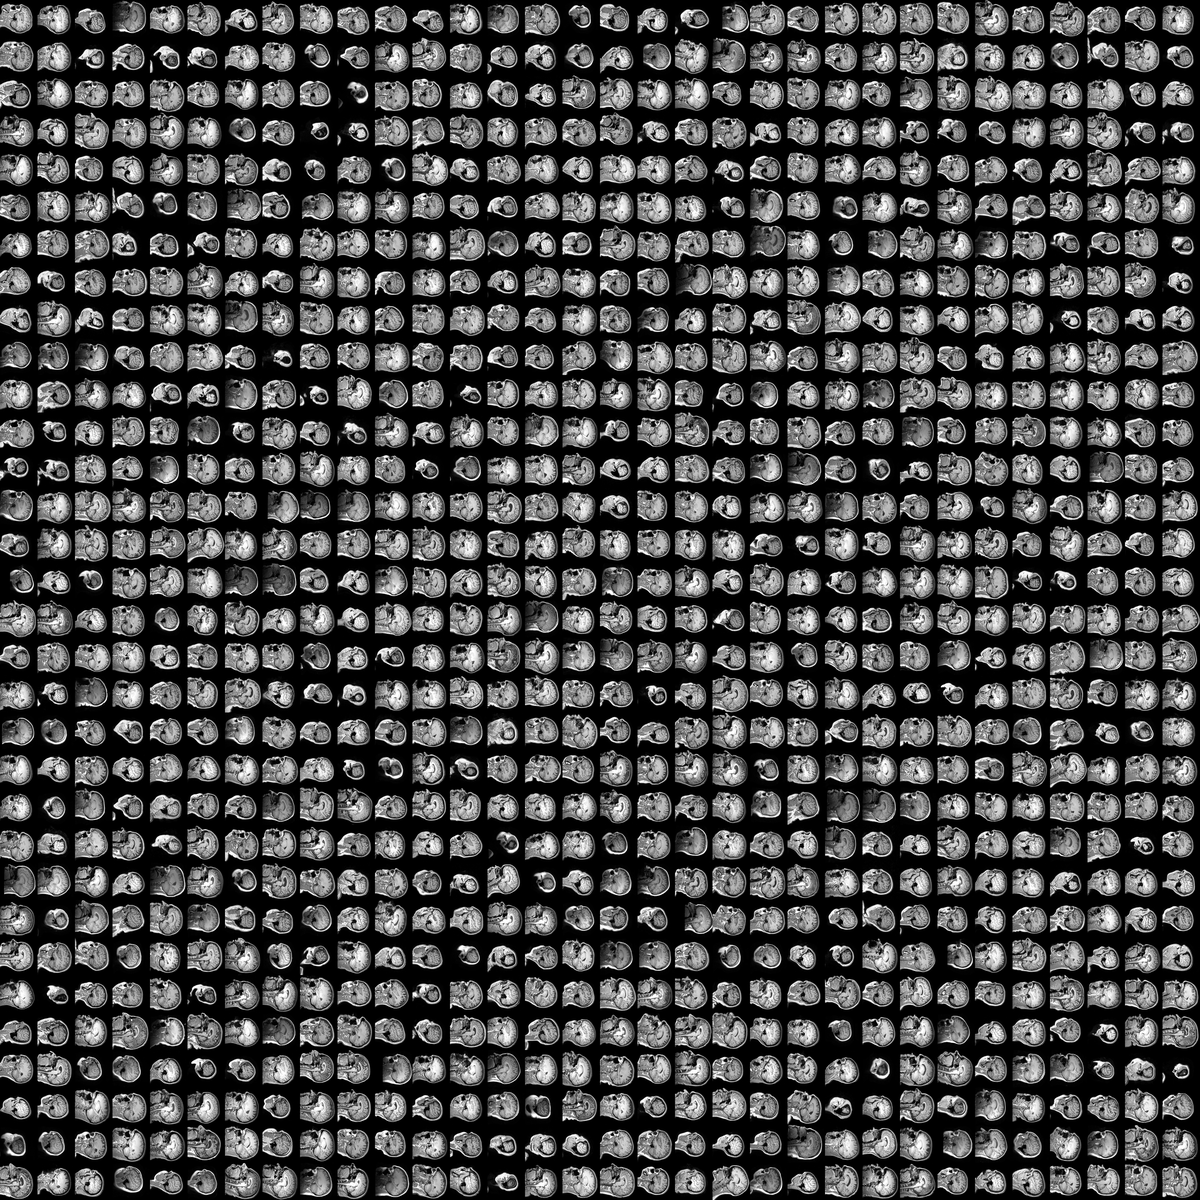
\includegraphics[width=0.82\textwidth]{figures/stylegan2_reals_preview.png}
\caption{StyleGAN2 训练集中真实 MRI 切片样本网格}
\label{fig:stylegan2-reals}
\end{figure}

训练结束后，项目得到可加载的模型快照 \texttt{network-snapshot-010000.pkl}。平台能够读取该权重并生成 MRI 切片，说明权重加载、潜变量采样、生成器推理、图像张量转换和 PNG 保存等环节可以顺利衔接。对 StyleGAN2 结果的评价不放在临床诊断性能上，而是关注生成链路是否可用、输出是否可复现，以及生成切片能否继续支撑三维输入组织。

\section{二维切片生成结果分析}
平台生成的示例切片如图 \ref{fig:generated-slices} 所示。图像来自生成切片结果目录，由训练完成的 StyleGAN2 权重生成。不同随机种子对应不同潜变量输入，因此输出切片在灰度分布和结构形态上会出现差异。图中可以看到脑部 MRI 切片的基本轮廓和灰度层次，这说明平台推理模块能够正确调用训练权重，并把模型输出保存为可查看的图像结果。

\begin{figure}[H]
\centering
\begin{subfigure}{0.32\textwidth}
\centering
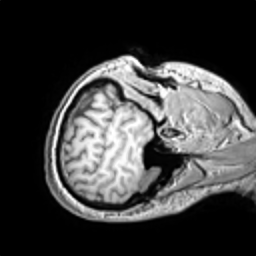
\includegraphics[width=\textwidth]{figures/generated_seed0123.png}
\caption{随机种子 123}
\end{subfigure}
\hspace{0.08\textwidth}
\begin{subfigure}{0.32\textwidth}
\centering
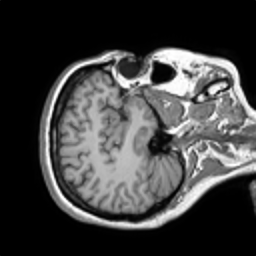
\includegraphics[width=\textwidth]{figures/generated_seed0042.png}
\caption{随机种子 42}
\end{subfigure}
\caption{StyleGAN2 生成的 MRI 切片示例}
\label{fig:generated-slices}
\end{figure}

从操作流程看，二维切片生成已经可以在平台中闭环完成。用户指定模型权重、生成数量、截断参数和随机种子后，后端完成潜变量采样、生成器推理、灰度图像转换和结果保存。截断参数 \texttt{truncation\_psi} 会影响图像稳定性和变化幅度，随机种子则保证同一参数下能够再次生成相同结果。该功能既能提供论文展示图，也能为连续切片序列和点云初始化提供输入。

\section{平台功能测试}
平台功能测试关注主要流程是否按预期运行。测试内容包括 FastAPI 后端接口、React 前端页面、数据预处理、模型训练入口、切片生成、连续序列生成、点云初始化、3DGS 结果展示和 AI 助手。测试结果显示，FastAPI 后端服务可以正常启动，React 前端可以访问平台页面；生成模块能够调用训练完成的权重输出 PNG 切片；点云初始化模块能够从切片目录生成 PLY 文件；3DGS 训练结果也能够以日志、渲染图像和点云文件形式归档。

\begin{table}[H]
\centering
\caption{平台主要功能测试结果}
\begin{tabular}{>{\raggedright\arraybackslash}p{3cm}>{\raggedright\arraybackslash}p{5.2cm}>{\raggedright\arraybackslash}p{4.8cm}}
\toprule
测试模块 & 测试内容 & 测试结果 \\
\midrule
数据预处理 & NIfTI 读取、轴向切片、归一化、缩放和 PNG 保存 & 已实现，可按数据目录批量处理 \\
模型训练 & 自动识别训练数据并启动 StyleGAN2 训练 & 已实现，训练结果已存在 \\
切片生成 & 加载 \texttt{.pkl} 权重并生成 PNG 图像 & 已通过，已有生成样例 \\
连续序列 & 潜空间插值得到连续切片序列 & 已实现，可用于三维展示 \\
点云初始化 & 将切片序列转换为 PLY 点云 & 已通过，已有 PLY 结果 \\
3DGS 重建 & 组织切片、点云、相机参数并完成训练输出 & 已通过，已有 checkpoint、点云和渲染结果 \\
FastAPI 后端 & 提供概览、生成、资产、任务、分析、报告和 AI 助手接口 & 已实现，可由 React 前端调用 \\
React 前端 & 提供仪表盘、生成、查看器、影像分析报告、可信性评估、任务、3D 和教学页面 & 已实现，可通过 Vite 本地服务访问 \\
AI 助手 & 参数说明和平台问答 & 已实现，包含本地解释逻辑和可选搜索接口 \\
\bottomrule
\end{tabular}
\end{table}

测试过程显示，平台已经具备毕业设计展示和实验复核所需的几项核心能力。第一，用户可以通过 React 前端生成二维切片并查看输出结果。第二，平台可以浏览连续 MRI 切片，并进入点云或体渲染页面查看三维资产。第三，FastAPI 后端可以维护任务状态、结果路径和日志信息，前端页面不需要直接调用底层训练脚本。第四，系统能够给出可信性提示和影像分析报告，用于说明生成结果的使用边界。需要说明的是，这些提示和报告只服务于教学解释与结果整理，不作为临床诊断依据。

为了更直观地展示平台实现效果，本文选取系统总览页、生成工作台、医学影像查看器和三维点云展示页作为功能截图。系统总览页汇总生成切片数量、连续序列数量、三维资产数量和当前风险提示状态，如图 \ref{fig:frontend-dashboard-generation}（a）所示。生成工作台用于配置模型权重、随机种子、截断参数和生成数量，并通过 FastAPI 后端调用 StyleGAN2 生成模块，如图 \ref{fig:frontend-dashboard-generation}（b）所示。这两个页面展示了平台从状态查看到二维切片生成的主要操作路径。

\begin{figure}[H]
\centering
\begin{subfigure}{0.48\textwidth}
\centering
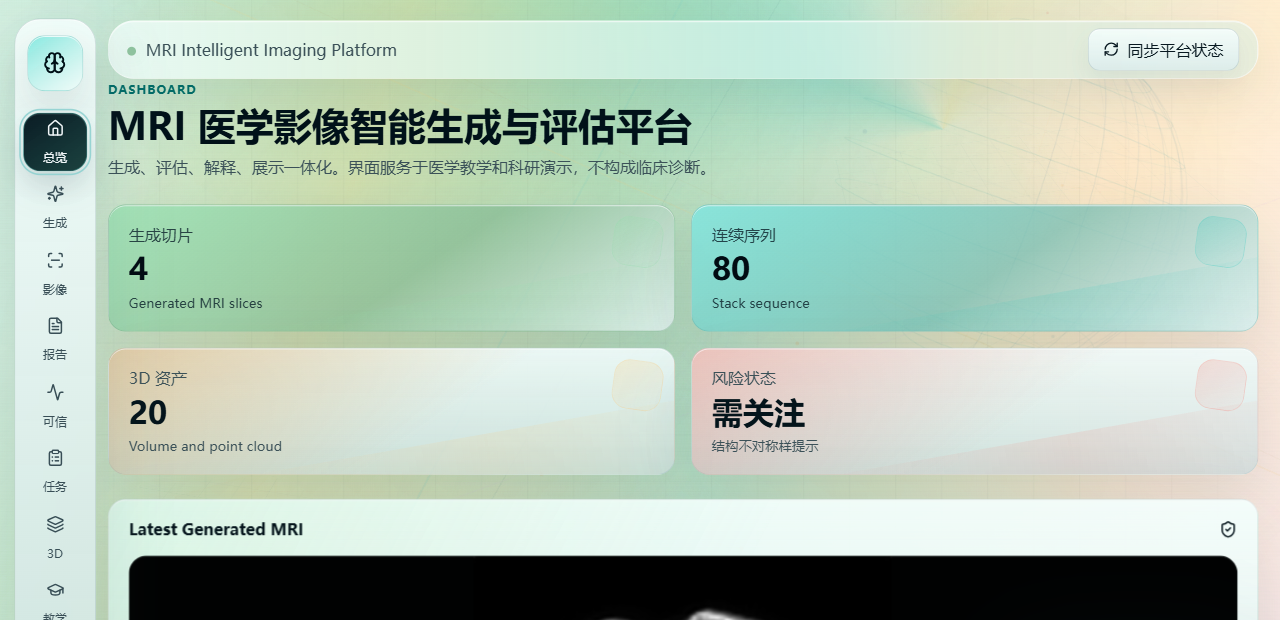
\includegraphics[width=\textwidth]{figures/frontend_dashboard.png}
\caption{系统总览页}
\end{subfigure}
\hfill
\begin{subfigure}{0.48\textwidth}
\centering
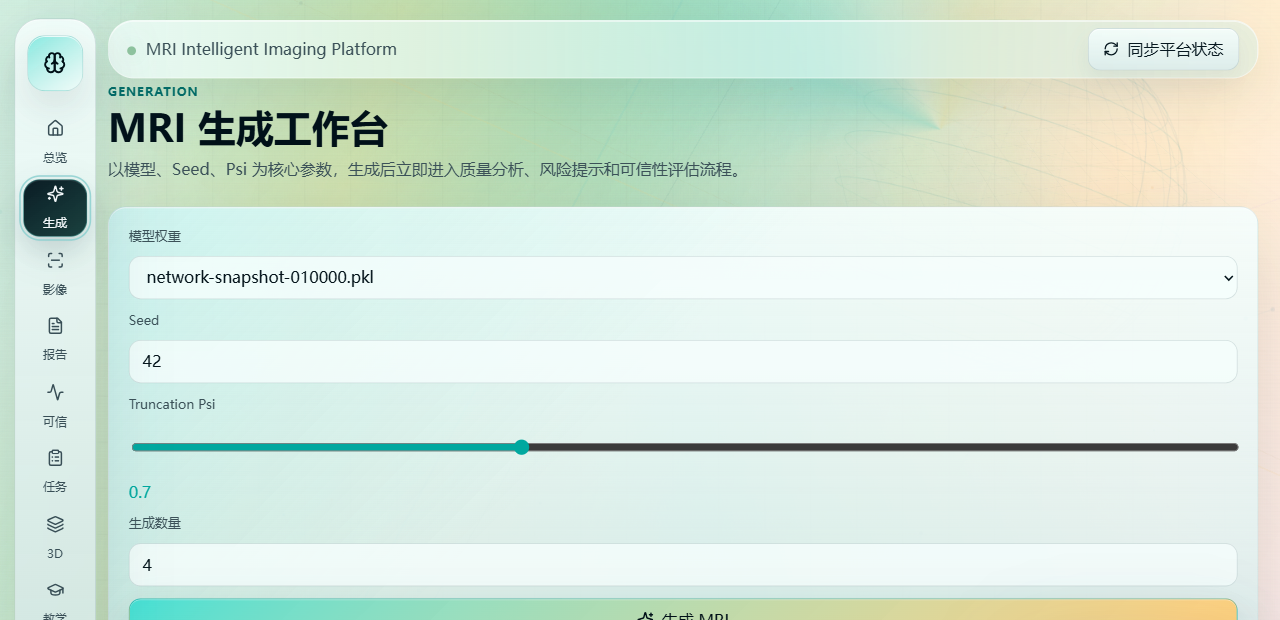
\includegraphics[width=\textwidth]{figures/frontend_generation.png}
\caption{生成工作台}
\end{subfigure}
\caption{React 前端系统总览与生成工作台页面}
\label{fig:frontend-dashboard-generation}
\end{figure}

医学影像查看器和三维点云展示页主要用于结果复核。医学影像查看器基于前端影像组件显示连续 MRI 切片，并提供窗位、窗宽、缩放和平移等交互能力，如图 \ref{fig:frontend-viewer-pointcloud}（a）所示。三维点云展示页用于加载 3DGS 或 PLY 结构资产，并以轻量化点云形式展示三维重建结果，如图 \ref{fig:frontend-viewer-pointcloud}（b）所示。通过这两个页面，用户可以从二维切片观察扩展到三维结构查看，较完整地展示本系统“生成、分析、三维表达和教学演示”的设计目标。

\begin{figure}[H]
\centering
\begin{subfigure}{0.48\textwidth}
\centering
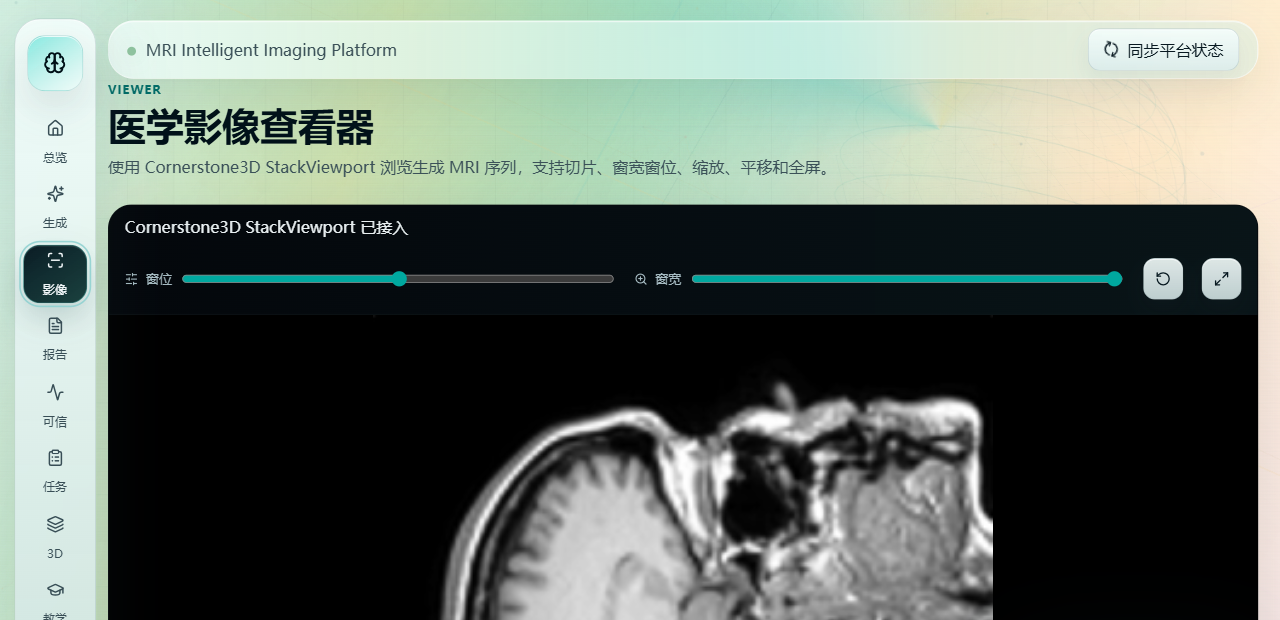
\includegraphics[width=\textwidth]{figures/frontend_viewer.png}
\caption{医学影像查看器}
\end{subfigure}
\hfill
\begin{subfigure}{0.48\textwidth}
\centering
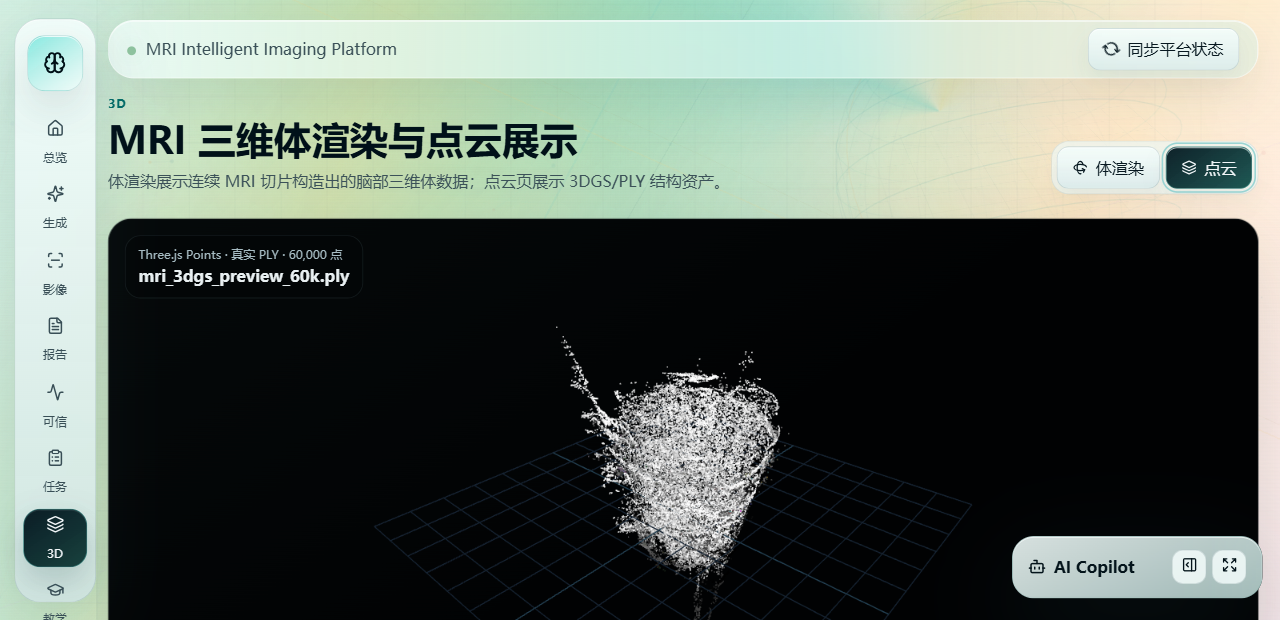
\includegraphics[width=\textwidth]{figures/frontend_pointcloud.png}
\caption{三维点云展示页}
\end{subfigure}
\caption{React 前端影像查看与三维点云展示页面}
\label{fig:frontend-viewer-pointcloud}
\end{figure}

三维页面还提供体渲染模式。该模式从连续 MRI 切片构建体数据，并通过阈值和透明度参数调节显示效果，如图 \ref{fig:frontend-volume} 所示。体渲染更适合观察连续切片形成的整体空间形态，点云模式则更适合展示 3DGS 或 PLY 结构资产。两种模式面向同一组三维结果，但观察侧重点不同。

\begin{figure}[H]
\centering
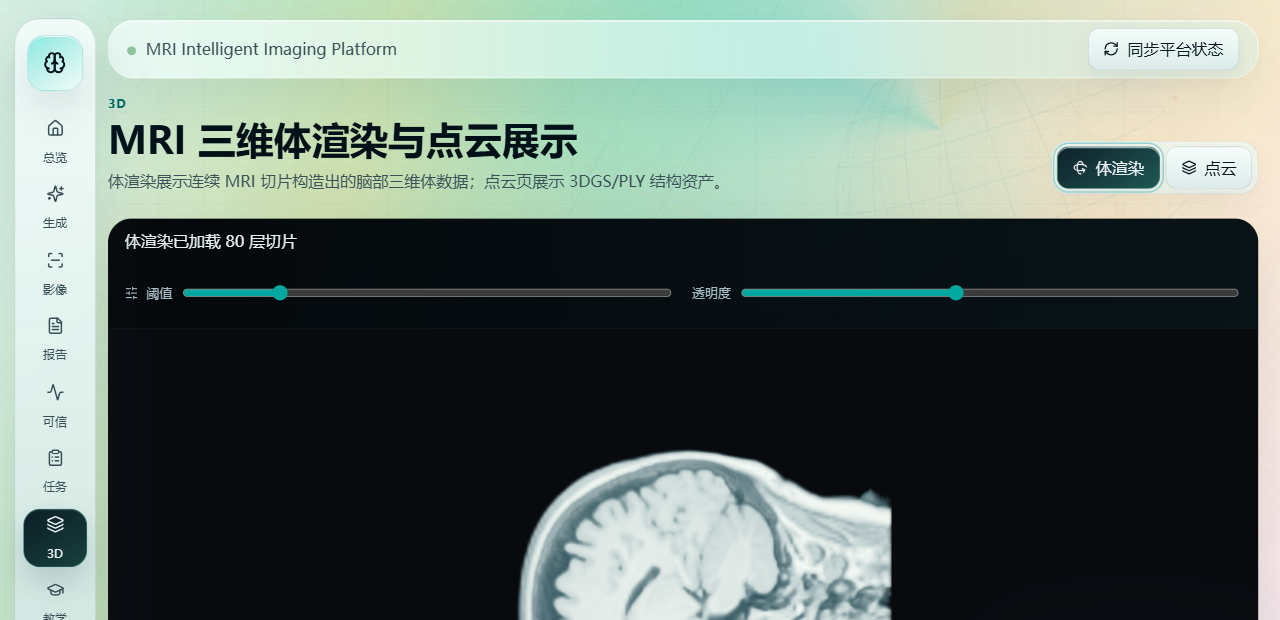
\includegraphics[width=0.82\textwidth]{figures/frontend_volume.png}
\caption{React 前端三维体渲染页面}
\label{fig:frontend-volume}
\end{figure}

报告页面和可信性评估页面用于解释生成结果。报告页面可以根据当前图像生成质量、结构、风险提示和教学说明，如图 \ref{fig:frontend-report-trust}（a）所示。可信性评估页面从真实性、多样性、非记忆性和解剖合理性等角度展示证据，如图 \ref{fig:frontend-report-trust}（b）所示。这两类页面不直接参与模型训练，但可以帮助用户理解生成结果的可靠性边界。

\begin{figure}[H]
\centering
\begin{subfigure}{0.48\textwidth}
\centering
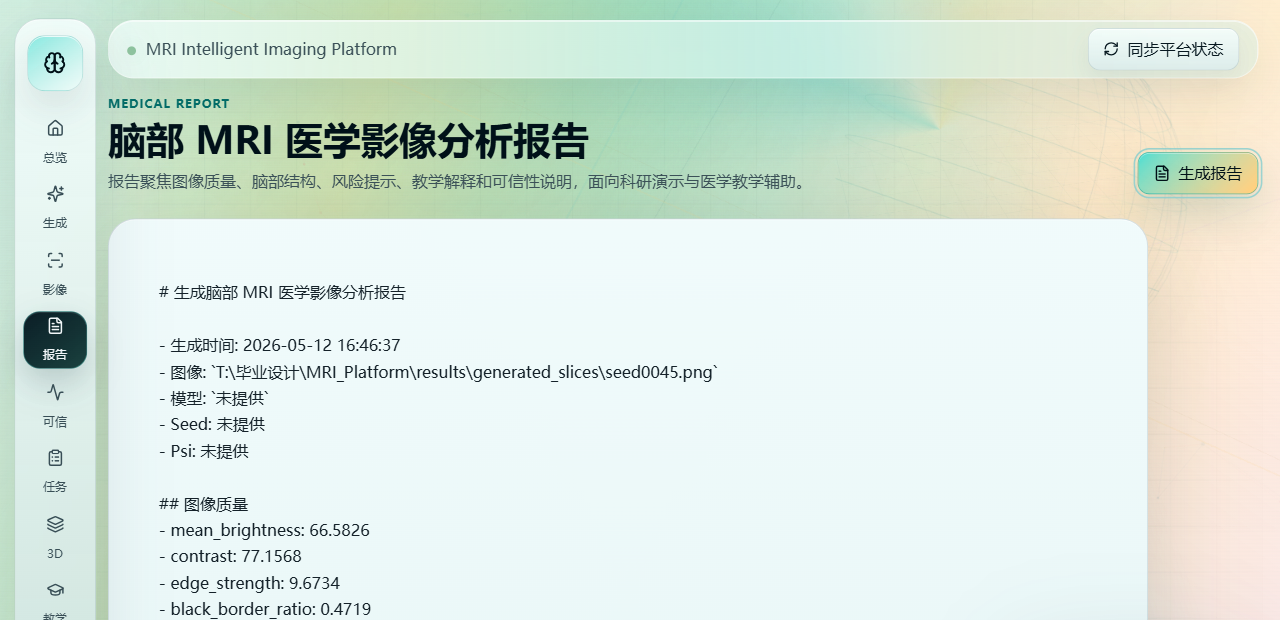
\includegraphics[width=\textwidth]{figures/frontend_report.png}
\caption{医学影像分析报告}
\end{subfigure}
\hfill
\begin{subfigure}{0.48\textwidth}
\centering
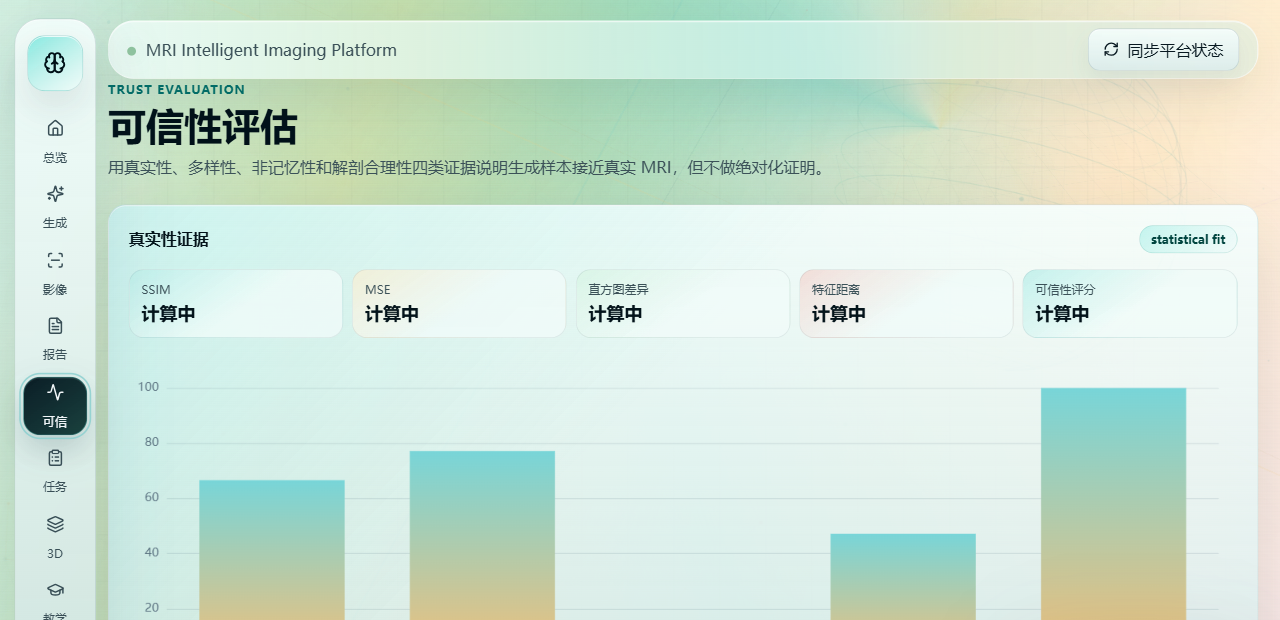
\includegraphics[width=\textwidth]{figures/frontend_trust.png}
\caption{可信性评估}
\end{subfigure}
\caption{React 前端报告生成与可信性评估页面}
\label{fig:frontend-report-trust}
\end{figure}

任务中心和医学教学中心用于支撑平台运行管理与答辩演示。任务中心记录生成、训练、评估、报告和三维任务的状态、输出路径和日志信息，如图 \ref{fig:frontend-tasks-education}（a）所示。医学教学中心把 MRI 基础、生成参数、质量指标和风险案例整理成交互式教学模块，如图 \ref{fig:frontend-tasks-education}（b）所示。通过这两个页面，系统不只展示算法结果，也能说明任务追踪、过程复核和教学辅助等工程功能。

\begin{figure}[H]
\centering
\begin{subfigure}{0.48\textwidth}
\centering
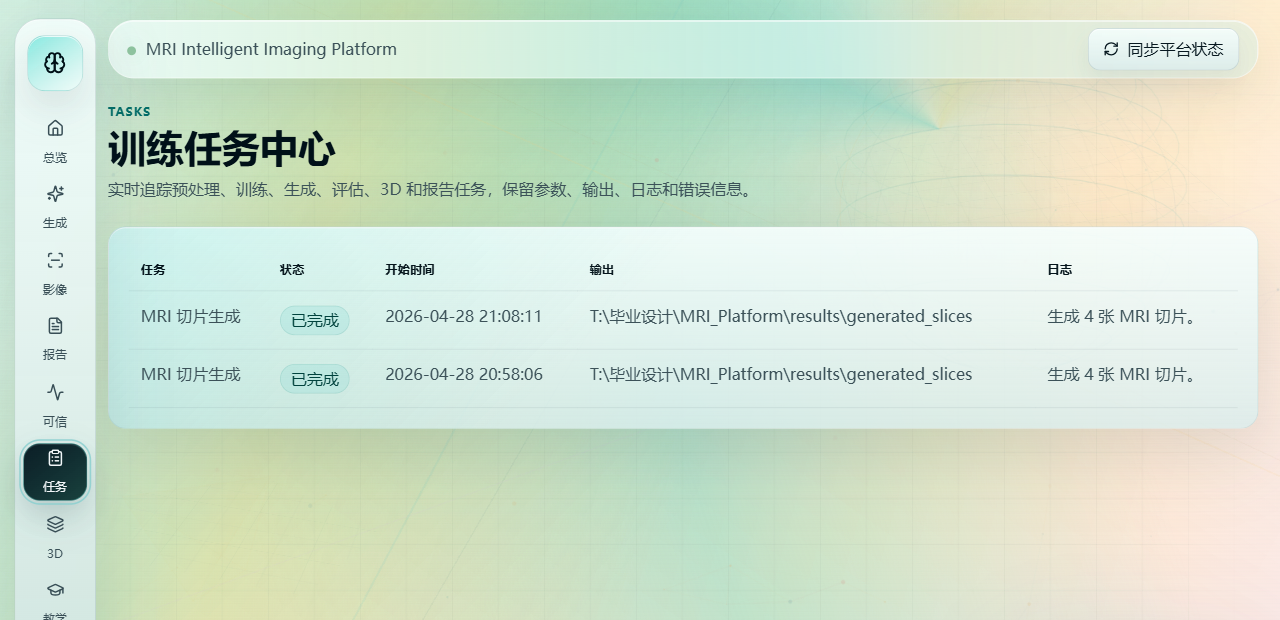
\includegraphics[width=\textwidth]{figures/frontend_tasks.png}
\caption{训练任务中心}
\end{subfigure}
\hfill
\begin{subfigure}{0.48\textwidth}
\centering
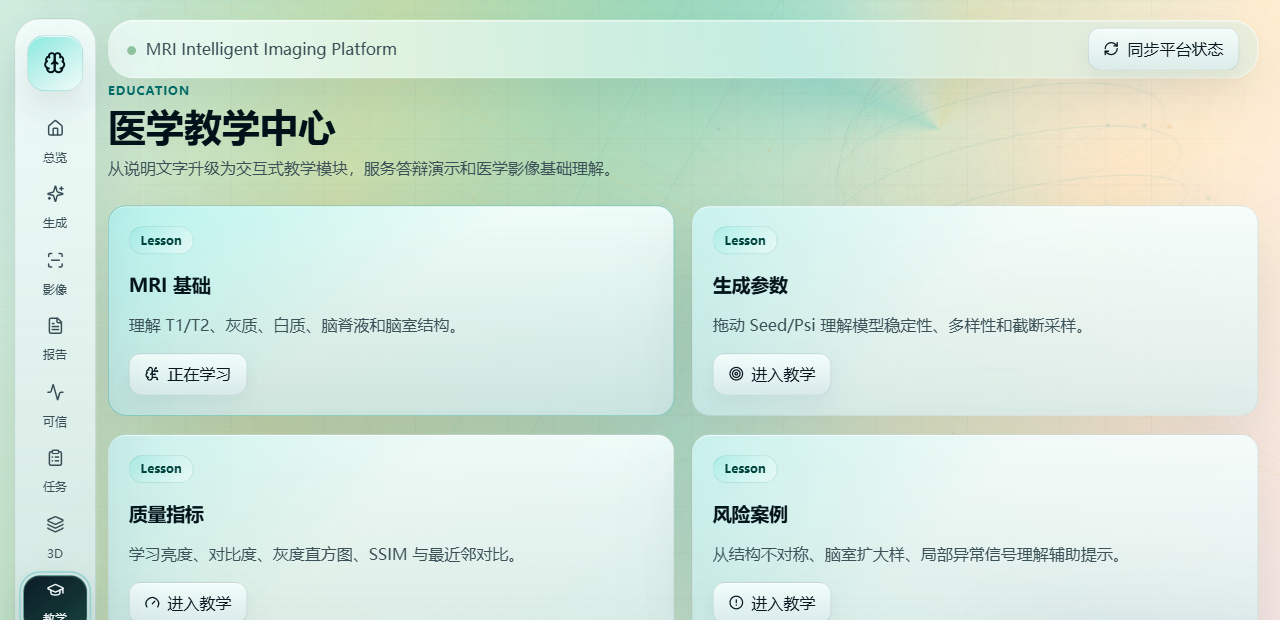
\includegraphics[width=\textwidth]{figures/frontend_education.png}
\caption{医学教学中心}
\end{subfigure}
\caption{React 前端任务管理与医学教学页面}
\label{fig:frontend-tasks-education}
\end{figure}

\section{点云初始化结果分析}
点云初始化结果由 \texttt{init\_pcd.py} 生成，输出文件为 \texttt{init\_point\_cloud.ply}。该文件大小约 13 MB。PLY 文件头显示包含 477426 个顶点，每个顶点包含三维坐标和 RGB 颜色信息。点云预览如图 \ref{fig:init-point-cloud} 所示。

\begin{figure}[H]
\centering
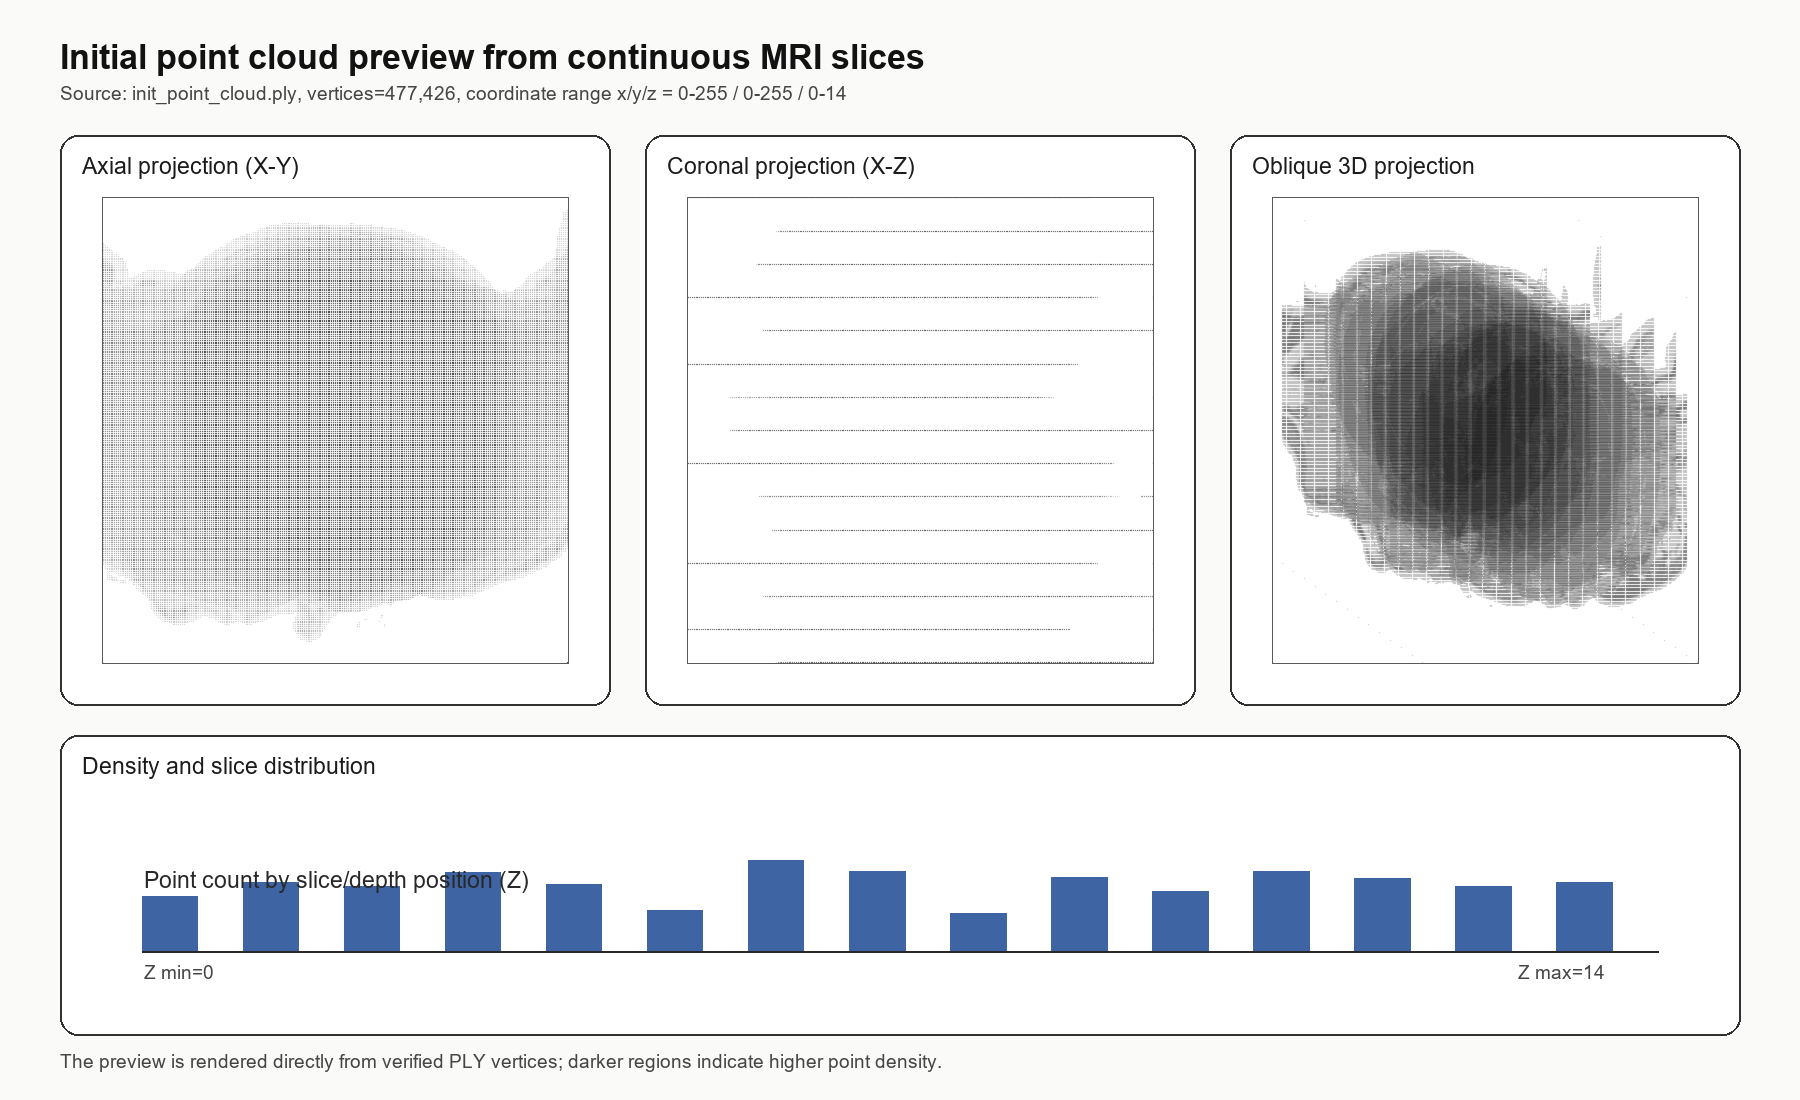
\includegraphics[width=0.82\textwidth]{figures/init_point_cloud_preview.png}
\caption{由连续 MRI 切片初始化得到的点云投影与密度分布预览}
\label{fig:init-point-cloud}
\end{figure}

该点云记录了二维切片进入三维空间的过程。每张切片对应一个 $z$ 轴位置，非背景像素被映射为空间点，像素灰度则被写入颜色强度。这样得到的点云既能作为 3DGS 三维重建输入，也能作为平台 2D/3D 对比展示的中间结果。相比只展示单张二维图，这一步提供了更明确的三维工程接口。

\section{3DGS 训练配置与重建结果}
3DGS 实验使用 180 张连续 MRI 切片作为监督图像，并以 300000 个点构建初始 PLY 点云。训练结果保存在 3DGS 主训练目录中。训练配置文件显示，模型采用三阶球谐函数表示颜色，输入图像目录为 \texttt{images}，数据设备为 CUDA。训练输出目录保存相机参数、checkpoint、训练日志、渲染结果和点云文件。

\begin{table}[H]
\centering
\caption{3DGS 训练主要参数与输出}
\begin{tabular}{>{\raggedright\arraybackslash}p{4.1cm}>{\raggedright\arraybackslash}p{8.2cm}}
\toprule
参数项 & 参数值或结果 \\
\midrule
训练切片数量 & 180 张 \\
训练图像分辨率 & $256\times256$ \\
初始点云规模 & 300000 点 \\
相机参数数量 & 180 个相机条目 \\
颜色表示 & 三阶球谐函数，\texttt{sh\_degree=3} \\
训练迭代次数 & 30000 轮 \\
最终 checkpoint & \texttt{chkpnt30000.pth} \\
最终点云 & 第 30000 轮输出 PLY 点云 \\
最终高斯点数量 & 556424 个 \\
前端预览点云 & 60000 点 \\
\bottomrule
\end{tabular}
\end{table}

训练过程中，系统在第 1000、3000、7000、15000 和 30000 轮记录训练集重建指标，也保存对应高斯点云。表 \ref{tab:3dgs-metrics} 给出了训练日志中的主要指标。随着迭代推进，L1 误差整体下降，PSNR 整体提高，说明三维高斯参数在切片监督下逐步逼近目标 MRI 切片分布。

\begin{table}[H]
\centering
\caption{3DGS 训练过程指标}
\label{tab:3dgs-metrics}
\begin{tabular}{cccc}
\toprule
迭代轮数 & L1 误差 & PSNR/dB & 说明 \\
\midrule
1000 & 0.0986 & 14.6051 & 初始优化阶段 \\
3000 & 0.0778 & 16.1066 & 结构逐步收敛 \\
7000 & 0.0675 & 16.8441 & 中期稳定优化 \\
15000 & 0.0579 & 17.9135 & 重建质量继续提升 \\
30000 & 0.0459 & 20.0909 & 最终训练结果 \\
\bottomrule
\end{tabular}
\end{table}

最新训练日志和前端展示摘要文件显示，3DGS 在第 30000 轮训练集评估中达到 L1 为 0.0459、PSNR 为 20.0909 dB。这组指标来自训练过程对 180 张监督切片的渲染重建评估，反映的是本平台实验中的重建一致性，并不能解释为医学诊断性能。训练指标变化如图 \ref{fig:3dgs-metrics-30000} 所示。

\begin{figure}[H]
\centering
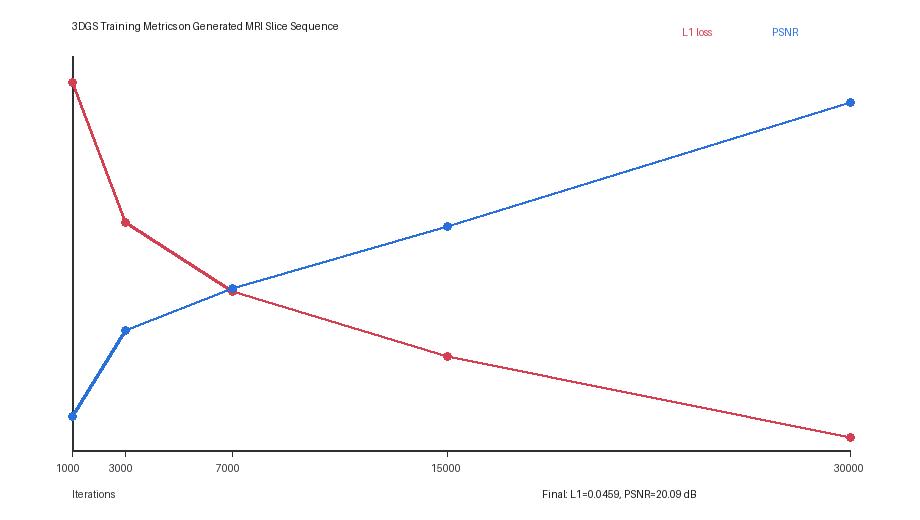
\includegraphics[width=0.9\textwidth]{figures/3dgs_metrics_30000.png}
\caption{3DGS 训练过程 L1 与 PSNR 指标变化}
\label{fig:3dgs-metrics-30000}
\end{figure}

从指标变化看，训练前期主要让整体轮廓和灰度分布逐步对齐，后期继续降低像素误差。这里的 PSNR 只说明渲染结果和监督切片之间更接近，并不能说明生成结果具备临床可用性。原因在于本实验输入是规则 MRI 切片序列，不是来自真实相机的多视角图像。本文把该指标作为工程训练过程的复核依据，而不是医学诊断性能指标。

第 30000 轮渲染切片与参考切片对比如图 \ref{fig:3dgs-comparison-30000} 所示。图中选取序列前部、中部和后部切片进行展示。渲染结果在脑部轮廓、主体灰度区域和层间变化趋势上与参考切片保持一致，但局部细节仍有一定平滑化现象。这与 MRI 灰度纹理、单序列输入约束和当前训练规模有关。

\begin{figure}[H]
\centering
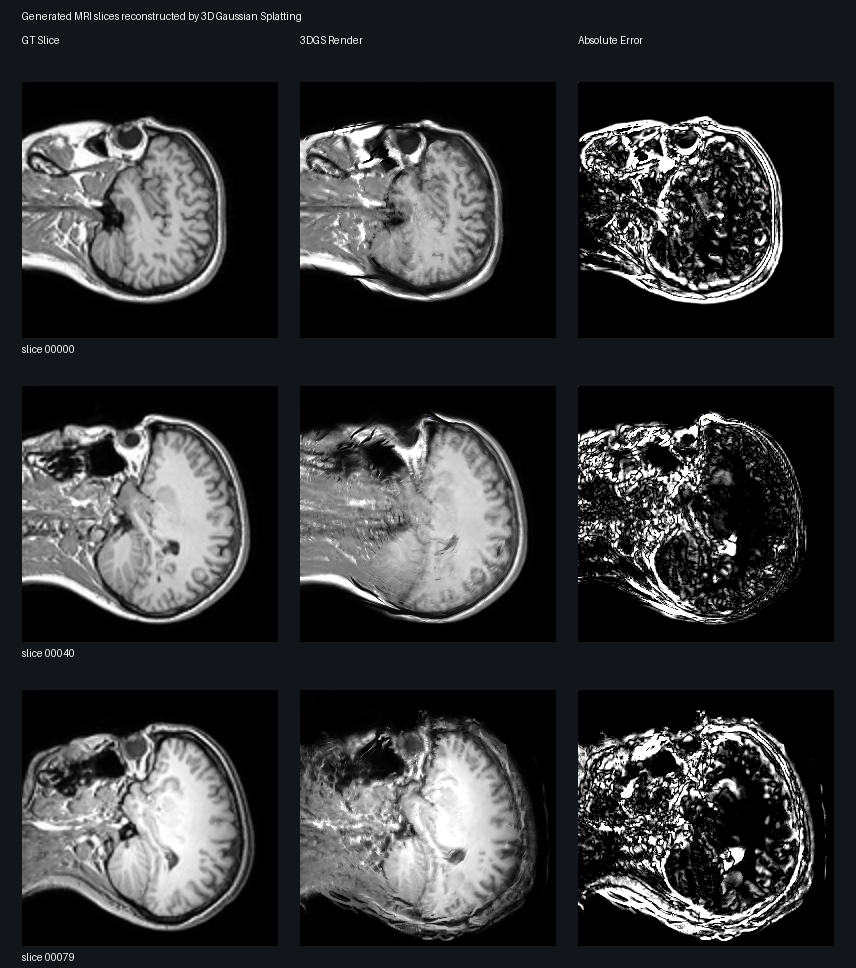
\includegraphics[width=0.82\textwidth]{figures/3dgs_slice_comparison_30000.png}
\caption{3DGS 第 30000 轮渲染切片与参考切片对比}
\label{fig:3dgs-comparison-30000}
\end{figure}

结合训练日志、checkpoint、点云文件和渲染结果可以确认，3DGS 模块已经完成训练闭环。该闭环从规则切片序列开始，最终输出可保存、可预览的三维高斯表达。输入点云从 300000 点优化为 556424 个高斯点，说明训练过程在初始空间结构基础上调整并扩展了三维表达。前端展示时，系统使用 60000 点预览点云降低浏览器加载压力，同时保留完整 PLY 文件作为实验产物。这样处理后，平台既能展示轻量化点云，也能保留完整训练结果用于复核。

\section{综合评价与局限性分析}
综合实验结果可以看到，项目已经跑通 MRI 数据预处理、StyleGAN2 二维生成、连续切片组织、点云初始化和 3DGS 三维训练结果展示等主要流程。StyleGAN2 部分留下了可加载权重和生成切片，3DGS 部分留下了训练日志、checkpoint、渲染图像和训练后点云。平台采用 FastAPI + React 架构，能够提供后端接口、前端页面、任务状态、影像查看和三维展示。就毕业设计要求而言，系统已经覆盖算法实现、工程集成、实验验证和可视化展示几个核心方面。

系统仍有可以继续改进的地方。StyleGAN2 生成结果目前主要通过可视化和工程链路验证，缺少大规模样本统计和医学专家评价。3DGS 训练基于规则切片相机和单序列灰度图像，已经能够形成可展示的三维表达，但局部组织边界仍有平滑化现象。平台目前主要以本地 FastAPI 服务和 Vite 前端运行，跨环境部署能力还可以通过统一配置、环境变量和容器化方式继续增强。

\chapter{结论与展望}

\section{结论}
本文围绕“基于 3DGS 与 StyleGAN2 的 MRI 医学图像拟生成平台的设计与实现”开展工作。课题最终完成了 MRI 数据预处理、二维切片生成、连续切片组织、点云初始化、3DGS 训练结果接入和前后端平台展示。整个工作不是单独复现某个算法，而是把多个原本分散的步骤整理成一条可以运行、可以展示、可以复核的工程链路。

具体来看，平台已经实现四项主要功能。第一，系统可以读取 NIfTI 格式 MRI 数据，并完成切片提取、灰度归一化、尺寸调整、低信息切片过滤和训练数据整理。第二，项目基于 StyleGAN2-ADA 完成二维 MRI 切片生成模型训练，并把训练权重接入平台推理流程。用户可以通过随机种子和截断参数生成可复现的切片结果。第三，项目把连续切片序列转换为 PLY 初始点云，并构建规则相机参数，使 3DGS 可以在该输入上完成三维表达实验。第四，平台采用 FastAPI 和 React 实现前后端分离，整合结果概览、切片生成、医学影像查看、任务管理、三维展示和 AI 助手等页面。

本课题的创新点主要体现在工程适配和流程集成上。StyleGAN2、StyleGAN2-ADA 和 3DGS 的基础算法来自已有公开研究，本文不把算法原理本身作为原创贡献。本文的工作在于把 StyleGAN2 的二维生成能力接入 MRI 切片流程，把连续切片组织为点云和 3DGS 输入，并把训练、推理、结果管理和可视化统一到 FastAPI + React 平台中。这样处理后，算法结果不再只停留在命令行和离线文件中，而是可以通过页面查看、解释和复核。

实验结果表明，平台已经具备教学演示和实验复核所需的基本能力。StyleGAN2 训练链路形成了可加载权重，平台可以基于该权重生成 MRI 切片。3DGS 部分在 180 张连续切片监督下完成训练，并输出三维高斯模型、渲染结果和训练指标。第 30000 轮训练达到 L1 为 0.0459、PSNR 为 20.0909 dB，完整点云包含 556424 个高斯点，前端预览点云包含 60000 个点。这些结果说明，平台已经把二维生成、三维表达和结果展示连接成可操作流程。

本文也明确限定了平台的使用边界。当前系统主要用于教学演示、毕业设计展示和工程实验验证，不用于临床诊断。实验数据以脑部 T1 MRI 为主，数据类型和病例来源仍然有限。3DGS 部分使用规则切片相机和单序列灰度图像，能够形成可展示的三维表达，但还不能完整代表真实医学空间结构。评价方面，本文使用 L1、PSNR 和可视化对比进行分析，尚未加入医学专家评价、下游任务验证和更全面的医学可信性评估。

\section{展望}
后续工作可以先从三维表达继续完善。当前系统使用规则相机参数完成 3DGS 训练，能够支撑工程展示，但还没有充分利用 NIfTI 中的真实体素间距、层厚和空间方向信息。后续可以把这些信息加入相机参数构建过程，并尝试层间连续性约束、结构平滑约束和高斯点裁剪策略，让三维表达更加接近 MRI 体数据本身的空间关系。

评价体系也需要进一步补充。当前论文主要使用 L1、PSNR 和可视化对比来说明训练过程。后续可以加入 SSIM、FID、LPIPS、分割一致性或下游任务性能等指标。对于医学图像生成任务，还需要医学专业人员参与主观评价，从结构合理性、解剖一致性和教学可用性等角度检查生成结果。

平台工程方面也还有提升空间。当前系统已经能够通过本地 FastAPI 服务和 React 前端完成主要功能展示，但运行时仍依赖本地模型路径、数据路径、GPU 环境和外部接口配置。后续可以通过配置文件、环境变量、任务队列和容器化部署规范运行环境。对于耗时较长的训练任务，还可以加入更完善的日志追踪、失败恢复和资源监控功能。

应用场景方面，本文主要围绕脑部 T1 MRI 切片展开。后续可以扩展到多序列 MRI、CT 或其他公开医学图像数据集，也可以研究跨模态生成、数据增强和三维教学展示等任务。若未来能够获得更充分的数据、专家评价和伦理审查支持，平台可以继续作为医学图像生成方法比较、三维重建流程教学和医学人工智能实验课程的辅助工具。


\clearpage
\printbibliography[heading=bibintoc,title=参考文献]

\clearpage
\chapter*{附\quad 录}
\thispagestyle{thesis-main}
\addcontentsline{toc}{chapter}{\texorpdfstring{附\quad 录}{附 录}}
\markboth{成都信息工程大学学士学位论文}{成都信息工程大学学士学位论文}

\thesisbodyfont
\justifying

\noindent{\songti\bfseries 附录 A\quad 项目主要文件与实验产物}

本文涉及的工程代码与实验结果主要保存在项目目录 \thesispath{MRI_Platform} 中。后端入口文件为 \thesispath{backend/app/main.py}。该文件用于创建 FastAPI 应用，并挂载 API、WebSocket 和静态媒体路由。主要接口文件为 \thesispath{backend/app/api/routes.py}。前端入口文件为 \thesispath{frontend/src/main.tsx}，核心页面文件为 \thesispath{frontend/src/app/App.tsx}。MRI 数据预处理脚本为 \thesispath{src/preprocess_mri.py}。该脚本负责读取 NIfTI 体数据并导出 PNG 切片。点云初始化脚本为 \thesispath{src/init_pcd.py}。该脚本负责把连续切片序列转换为 PLY 点云文件。

StyleGAN2 相关训练配置和日志保存在主训练运行目录中。训练配置文件记录训练数据、分辨率、batch size、学习率和 ADA 参数。日志文件保存训练过程输出。可加载模型权重、训练样本网格和生成切片样例分别位于训练结果目录与生成结果目录。这些文件可用于复核第 6 章中的二维生成实验。

三维重建结果包括初始点云文件、3DGS 训练目录和平台展示材料。初始点云文件 \thesispath{init_point_cloud.ply} 包含 477426 个顶点。复核样例包含 31980 个顶点。3DGS 主训练结果位于 \thesispath{results/3dgs_runs/mri_bestcand80_200k_30000_20260428_081347} 目录。该目录包含 180 个相机参数、30000 轮训练日志、\thesispath{chkpnt30000.pth}、第 30000 轮输出点云以及渲染切片和参考切片。最新前端展示资产保存在 \thesispath{results/3dgs_frontend} 中，其中 \thesispath{summary.json} 记录最终 L1 为 0.0459、PSNR 为 20.0909 dB，\thesispath{mri_3dgs_preview_60k.ply} 包含 60000 个预览点。论文使用的 3DGS 指标曲线和切片对比图保存在 \thesispath{figures/3dgs_metrics_30000.png} 与 \thesispath{figures/3dgs_slice_comparison_30000.png} 中。上述材料共同支撑第 5 章系统实现和第 6 章测试分析中的主要结论。


\clearpage
\chapter*{致\quad 谢}
\thispagestyle{thesis-main}
\addcontentsline{toc}{chapter}{\texorpdfstring{致\quad 谢}{致 谢}}
\markboth{成都信息工程大学学士学位论文}{成都信息工程大学学士学位论文}

\thesisbodyfont
\justifying

在本课题完成过程中，我得到了老师、同学和家人的关心与帮助。在此，我向所有给予指导、支持和鼓励的人表示诚挚感谢。

衷心感谢指导教师何长春讲师。何老师在选题确定、研究思路梳理、系统实现和论文撰写过程中给予了耐心指导。也感谢人工智能学院各位老师在课程学习、科研训练和毕业设计阶段提供的帮助，使我能够将生成式人工智能、医学图像处理和平台开发等知识应用到本课题中。

感谢数派（成都）数据科技有限公司在毕业设计过程中提供的算力支持。StyleGAN2 和 3DGS 的训练对显存、计算时间和运行环境稳定性都有较高要求。相关算力资源为模型训练、结果生成和实验复核提供了重要保障，也使本文能够较完整地完成从二维 MRI 切片生成到三维表达与平台展示的实验流程。

感谢家人和同学在学习与生活中的陪伴、鼓励与支持。正是这些帮助让我能够在毕业设计过程中持续推进系统开发、实验整理和论文写作，并最终完成本课题研究。\par

\vspace{0.5\baselineskip}

\noindent 作者简介：\par

\begingroup
\renewcommand{\arraystretch}{1.4}
\noindent\begin{tabular*}{\textwidth}{@{}p{0.46\textwidth}@{\extracolsep{\fill}}p{0.46\textwidth}@{}}
姓名：黎曜玮 & 性别：男 \\
出生年月：{\tnr 2004}年{\tnr 7}月{\tnr 24}日 & 民族：汉族 \\
\multicolumn{2}{@{}l@{}}{E-mail：{\tnr 17781088366@163.com}} \\
\end{tabular*}
\endgroup\par


\end{document}
